\documentclass[10pt]{article}
% Named draft for advisor review. Use \usepackage{tmlr} for blind submission.
% The official style file is included unchanged.
\usepackage[preprint]{tmlr}
\usepackage[utf8]{inputenc}
\usepackage{amsmath,amssymb}
\usepackage{booktabs,longtable,array}
\usepackage{graphicx}
\usepackage{hyperref}
\usepackage{url}
\usepackage{placeins}
\hypersetup{pdftitle={Mixed-activation layers: Robustness first, accuracy at width},pdfauthor={Barkev Sarkli and Rahim Dehkharghani},colorlinks=true,linkcolor=blue,citecolor=blue,urlcolor=blue}
\newcommand{\TR}{tanh + ReLU}
\newcommand{\TL}{tanh + leaky-ReLU}
\newcommand{\SR}{sigmoid + ReLU}
\title{Mixed-activation layers:\newline Robustness first, accuracy at width}
\author{\name Barkev \c{S}arkl\i\ \email barkev.sarkli@stu.khas.edu.tr\\
\addr Undergraduate student
\AND
\name Rahim Dehkharghani}
\begin{document}
\maketitle
\begin{center}\small Draft for advisor review --- 1 October 2026\end{center}

\begin{abstract}
A neural network can reach high accuracy and then lose it during training. We test whether fixed mixed-activation layers reduce this failure in small fully connected networks on MNIST and CIFAR-10. The main tests use six widths, seven activation choices, and 30 seeds per setting; tuning uses six separate seeds. On MNIST at width 128 and learning rate 0.03, all 30 ReLU runs end below 15\% validation accuracy, while no tanh--ReLU run does. Mean final scores are 10.61\% and 96.76\%, with no added trainable parameters. Online loss traces show distinct forms of training failure. The gain depends on the rule used: the upper tested rate with no run losing more than ten percentage points rises from 0.02 to 0.03, while the looser near-chance rule permits large losses at 0.05. The hybrid's best sampled rate also shifts upward, so higher usable rates do not alone show a wider range relative to that best rate. Tuning data show that protection weakens at large widths and is lost on CIFAR-10 at widths 256 and 512. At large widths, mixed models can match strong accuracy controls, but we find no clear general accuracy gain after tuning. These results support a setting-specific training-stability benefit and separate it from accuracy, width, and loss-function effects.
\end{abstract}

\section{Introduction}
Most neural networks use the same activation function for all neurons in a hidden layer. This is a simple design choice, but it also gives those neurons the same type of response. ReLU is linear for positive inputs and zero for negative inputs. Tanh has both positive and negative outputs, but its output stays between $-1$ and $1$. Using both functions in the same layer may change how the network responds to large training steps.

We study this question through a fixed assignment of activation functions to neurons. Each neuron uses one function throughout training. The assignment adds no learned gates or extra weights. We call such a layer a \emph{mixed} or \emph{hybrid} layer. A layer in which every neuron uses the same function is a \emph{single-function} layer.

Our main focus is \emph{training stability}: whether a network keeps useful accuracy when the learning rate changes or training continues. This meaning is narrower than resistance to noisy images, attacks, or changes in the test data. We do not test those forms of robustness. We also separate training stability from best test accuracy. A model may have a wider useful learning-rate range without giving a higher score after careful tuning.

The study uses a two-hidden-layer multilayer perceptron (MLP). We compare four single functions and three mixed pairs on two image tasks. We change width, learning rate, activation share, mask layout, and the loss/output pair. This simple network makes the comparisons easier to read. It is not intended to compete with the best image models.

The paper has three main findings. First, a 50:50 tanh--ReLU split can prevent late loss of accuracy in MNIST runs where ReLU fails. Second, avoiding near-chance failure and keeping high accuracy are different outcomes; leaky-ReLU is a useful control for this reason. Third, the benefit depends on the dataset and training setup. Careful learning-rate selection removes most of one apparent test-accuracy gain. These limits are part of the result.

\section{Related work}
Activation choice and weight scale are closely linked. \citet{glorot2010} studied how activation outputs and gradients affect learning. \citet{glorot2011} showed the value of rectifier units, including their sparse zero outputs. \citet{he2015} developed an initialization rule that accounts for rectifier functions. These works support checking both activation choice and initialization when studying training stability.

Inactive ReLU units are another possible source of failure. \citet{lu2019} studied dying ReLU networks and ways to change initialization. Our MNIST loss traces and nearly single-class predictions are consistent with this type of failure after useful learning. We do not measure hidden-unit activity, so these observations support a hypothesis rather than establish a dead layer.

Using different activation functions within a network is not a new idea. \citet{hagg2017} used an evolutionary search to select activation functions for individual neurons, along with network structure and weights. \citet{manessi2018} learned combinations of base functions during training. Our design fixes the network size and assigns one function to each neuron before training. We study the training behavior of this fixed assignment with single-example stochastic gradient descent (SGD). We make no claim to introduce mixed activations or the idea of an activation share for the first time.

Finally, the choice of tuning rule can change a model comparison. \citet{cawley2010} describe how model selection can affect reported performance. We therefore show both the original tuning rule and a check that matches tuning to the model checkpoint used at test time.

\section{Network and experiment setup}
\subsection{Fixed activation assignments}
The network has the form $D\rightarrow H\rightarrow H\rightarrow 10$. Here $D$ is the input size and $H$ is the width of each hidden layer. For neuron $i$ in layer $l$, let $z_{l,i}$ be its weighted input. A fixed binary mask $m_{l,i}$ sets its function:
\begin{equation}
h_{l,i}=\begin{cases} f_1(z_{l,i}),&m_{l,i}=0,\\f_2(z_{l,i}),&m_{l,i}=1.\end{cases}
\qquad
\rho_l=\frac{1}{H}\sum_{i=1}^{H}m_{l,i}.
\label{eq:mask}
\end{equation}
We call $\rho_l$ the \emph{activation allocation ratio}: the share of neurons assigned to the second function. This is a definition for this study, not a claim of a new general concept. The main tests use $\rho_l=0.5$ in both layers. A neuron does not compute a weighted sum of tanh and ReLU.

The main mask spreads the two functions across each layer. The code calls this layout \texttt{interleave}. We also test a block layout and a shuffled layout. The ratio controls how many neurons use each function; the layout controls their positions. Figure~\ref{fig:network} shows the fixed assignment.

\begin{figure}[htbp]
\centering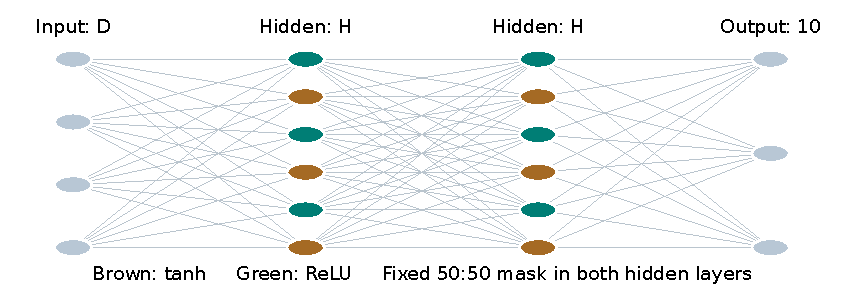
\includegraphics[width=0.94\linewidth]{figures/network.pdf}
\caption{The tested MLP and a 50:50 tanh--ReLU mask. The drawing shows only a few units. Both hidden layers have the same width and activation share. The output layer uses one common output rule.}
\label{fig:network}
\end{figure}

We use ReLU, leaky-ReLU, tanh, and sigmoid as single-function controls. The mixed pairs are \TR, \TL, and \SR. Leaky-ReLU has negative-side slope 0.1. These choices let us compare each mixed pair with both of its parent functions.

\subsection{Data and training}
MNIST contains digit images \citep{lecun1998}. In these runs, a fixed shuffle of its 60,000-image training file gives 45,000 training, 5,000 validation, and 10,000 test images. Thus our MNIST test scores do not use the official test set. CIFAR-10 uses 45,000 training and 5,000 validation images from the standard training set and the official 10,000-image test set \citep{krizhevsky2009}. The split seed is 12345 and is shared by all model seeds. Input pixels are scaled to $[0,1]$; no image augmentation is used.

Each run uses 40 epochs of SGD with one image per update, a fixed learning rate, and a shuffled image order each epoch. We test $H\in\{12,32,64,128,256,512\}$. The main loss is cross-entropy (CE), with linear output scores followed by softmax. We also test the implemented mean squared error (MSE) loss with sigmoid outputs at $H=64$ and $128$ on MNIST.

Weights are drawn from $U(-1/\sqrt{n},1/\sqrt{n})$, where $n$ is the input count of the layer, and biases start at zero. The resulting weight variance is $1/(3n)$. This is six times smaller than the standard ReLU He variance $2/n$ \citep{he2015}. We keep this implemented scale common to all models; it should not be read as the best scale for each activation. The code clips each loss derivative with respect to a neuron's weighted input to $[-10,10]$.

\begin{table}[htbp]\centering
\caption{Completed experiment groups. Counts exclude repeated CSV header lines.}
\label{tab:inventory}\small
\begin{tabular}{@{}llrr@{}}\toprule
Group & Scope & Seeds per cell & Recorded rows\\\midrule
Main CE tests & Two datasets, six widths, seven models & 30 & 2,520\\
CE tuning & Eight learning rates per main setting & 6 & 4,032\\
Learning-rate tests & MNIST 64/128; CIFAR-10 128 & 30 & 6,300\\
Ratio and layout & MNIST 128; two mixed pairs & 30 & 300\\
MSE tests & MNIST 64/128; three models & 30 & 180\\
MSE tuning & Eight learning rates per MSE setting & 6 & 288\\\midrule
Total & 32 CSV files & & 13,620\\\bottomrule
\end{tabular}
\end{table}

\subsection{Tuning and checkpoint selection}
Learning-rate tuning uses seeds 101--106. Test runs use seeds 1--30. The tuning grid is
\begin{equation}
\mathcal{G}_{\rm tune}=\{0.0001,0.0003,0.001,0.003,0.01,0.03,0.1,0.3\}.
\end{equation}
The original rule selects the rate with the highest mean \emph{final} validation accuracy. The MNIST evaluation grids at widths 64 and 128 add 0.005, 0.02, and 0.05. The CIFAR-10 evaluation grid at width 128 uses the eight tuning rates. Each evaluation rate has 30 seeds per model.

The runner saves the first epoch that reaches the highest validation accuracy. We call this the \emph{selected checkpoint}, meaning the saved model state at that epoch. It is tested after training ends. The final epoch is also tested. All 40 epochs are completed, so checkpoint selection does not reduce the training time. Unless stated otherwise, test scores in this paper use the selected checkpoint. Final validation scores are used to study loss of performance during training. We do not choose between endpoints based on test accuracy.

Table~\ref{tab:inventory} lists the data. There are 690 repeated job identities across groups. In particular, some learning-rate tests repeat main runs. We never count these as extra independent seeds. Both test confusion matrices reproduce their saved accuracy and macro-F1 values to the precision in the CSVs. All validation curves have 40 entries and match the saved best score and epoch. All recorded statuses are \texttt{ok}; this field alone is not a full numerical check.

\subsection{Matched seeds and loss logging}
In the inspected implementation, interleave and block masks use no random draws. At a fixed dataset and width, the same seed therefore gives the same starting weights and per-epoch image order across single-function models, these mask layouts, ratios, and learning rates. The main ReLU--tanh--ReLU contrasts have this matched design. The random layout is the exception: its mask shuffle changes the random stream before weights and image orders are made. The source-to-AWS-binary limit noted below still applies.

The logged epoch loss is an average of per-image losses collected before each SGD update. We call it \emph{online training loss}: it combines predictions from changing model states within an epoch. CE logging also clips the true-class probability below at $10^{-12}$. The loss is not a fixed-checkpoint training or validation loss, and it should not be combined with end-of-epoch validation accuracy to infer exact prediction confidence.

\subsection{Measures and uncertainty}
For a run with validation accuracy $v_t$ at epoch $t$, we report
\begin{equation}
v_{\rm peak}=\max_{1\leq t\leq40}v_t,\qquad
d=v_{\rm peak}-v_{40},\qquad
F=\mathbb{1}[v_{40}<15].
\label{eq:failure}
\end{equation}
The drop $d$ is measured in percentage points (pp). The flag $F$ marks final accuracy close to chance on a ten-class task. The 15\% threshold was chosen during analysis and is a descriptive check, not a universal rule. A large drop can still matter when the final score is above 15\%.

We use three learning-rate range summaries. The first keeps sampled rates whose mean final validation score is within 1 pp of that model's own best grid mean. The second keeps sampled rates with no final score below 15\%. The third requires no run to lose more than 10 pp from peak to final validation accuracy. For each rule we report the widest consecutive set of passing grid points, measured by its log span. Small drops alone do not imply useful learning: an always-poor model can also pass the third rule. These summaries do not establish behavior at untested rates. We also count scores below 15\% at any logged epoch, including epoch 1, when describing CIFAR-10. Both thresholds were chosen after inspecting the data.

Test accuracy counts correct labels. Macro-F1 gives each class the same weight by averaging its F1 score. We give means and sample standard deviations (SDs) across 30 seeds. For a model difference, we match seed identifiers and resample the 30 pairs 10,000 times, using bootstrap seed 20260915. The 2.5th and 97.5th percentiles give a pointwise 95\% interval. We also apply the Holm correction to paired t-test p-values across 120 main checkpoint-accuracy comparisons. Six ratio tests form a separate correction group. These checks do not cover all prior choices or all figures. All uncertainty estimates are tied to one fixed data split and the observed tuning process.

\FloatBarrier
\section{Main result: resistance to late training collapse}
\subsection{A large effect on MNIST}
Figure~\ref{fig:curves} shows the main stability result. At $H=128$ and learning rate 0.03, ReLU reaches a mean peak validation score of 96.371\%, but ends at 10.611\%. Its mean loss from peak to final is 85.760 pp. The 50:50 tanh--ReLU model reaches 97.230\% and ends at 96.761\%, a loss of only 0.469 pp. All 30 ReLU runs end below 15\%; none of the mixed runs does.

\begin{figure}[htbp]\centering
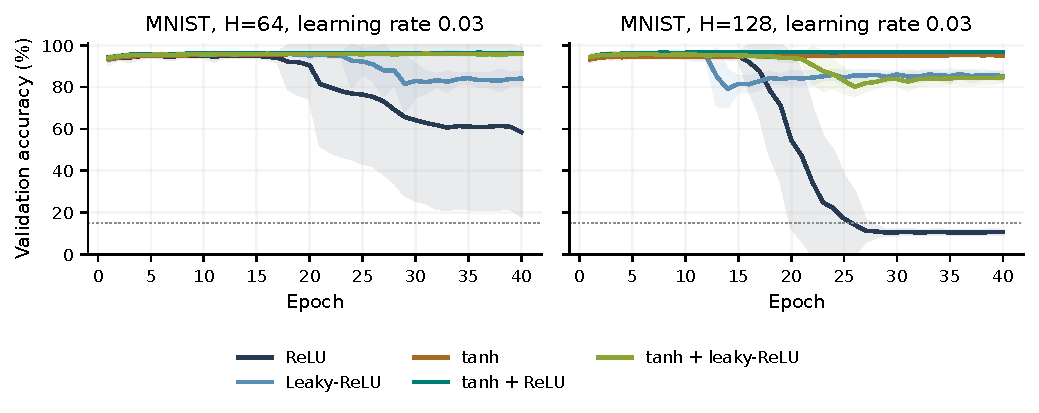
\includegraphics[width=\linewidth]{figures/training_curves.pdf}
\caption{Validation accuracy at learning rate 0.03 on MNIST. Lines are seed means and shaded bands are $\pm1$ seed SD, clipped to 0--100\%. The dotted line is the 15\% failure threshold. The tanh--ReLU model keeps high accuracy while ReLU loses it late in training. The wide ReLU band at H=64 reflects a mix of failed and useful runs.}
\label{fig:curves}\end{figure}

\begin{table}[htbp]
\centering
\caption{MNIST at learning rate 0.03. Each row has 30 seeds. The loss is peak minus final validation accuracy.}
\label{tab:stress}
\small
\begin{tabular}{@{}rlrrrr@{}}
\toprule
H & Model & Final acc. (SD) & Peak acc. & Loss (pp) & Below 15\% \\
\midrule
64 & ReLU & 58.431 (40.047) & 95.891 & 37.460 & 12/30 \\
64 & Leaky-ReLU & 84.005 (2.889) & 96.629 & 12.625 & 0/30 \\
64 & tanh & 95.907 (0.303) & 96.398 & 0.491 & 0/30 \\
64 & sigmoid & 97.558 (0.137) & 97.659 & 0.101 & 0/30 \\
64 & tanh + ReLU & 96.393 (0.302) & 96.861 & 0.468 & 0/30 \\
64 & tanh + leaky-ReLU & 95.689 (0.506) & 96.539 & 0.849 & 0/30 \\
64 & sigmoid + ReLU & 96.451 (0.261) & 96.870 & 0.419 & 0/30 \\
128 & ReLU & 10.611 (0.911) & 96.371 & 85.760 & 30/30 \\
128 & Leaky-ReLU & 85.228 (2.276) & 96.365 & 11.137 & 0/30 \\
128 & tanh & 95.111 (0.580) & 95.862 & 0.751 & 0/30 \\
128 & sigmoid & 98.031 (0.156) & 98.115 & 0.083 & 0/30 \\
128 & tanh + ReLU & 96.761 (0.258) & 97.230 & 0.469 & 0/30 \\
128 & tanh + leaky-ReLU & 84.633 (2.122) & 96.357 & 11.724 & 0/30 \\
128 & sigmoid + ReLU & 97.784 (0.189) & 97.884 & 0.100 & 0/30 \\
\bottomrule
\end{tabular}
\end{table}


At $H=64$, 12 of the 30 ReLU runs fail by the same rule. This gives a mean final score of 58.431\% and a very large SD of 40.047 pp. The mean alone hides two types of outcome. Tanh--ReLU gives 96.393\% with SD 0.302 pp and no near-chance runs. Table~\ref{tab:stress} includes all seven models, so the result is not based on one selected control.

Table~\ref{tab:onset} shows when the failures first appear. For ReLU at H=128, the first validation score below 15\% occurs between epochs 17 and 28, with a median of 21.5. At the final epoch, each of those ReLU runs predicts one class for at least 99.97\% of test images. Exactly 26 of 30 runs use only one predicted class; the other four use that class for 9,997--9,999 of 10,000 images. The most-used class holds, on average, 11.4\% of the mixed model's final test predictions. This supports late training collapse, rather than a network that never learned. It does not identify which hidden units caused the failure.

\begin{table}[htbp]
\centering
\caption{When failure first appears at MNIST learning rate 0.03. Class share uses final test predictions.}
\label{tab:onset}
\footnotesize
\begin{tabular}{@{}rllrr@{}}
\toprule
H & Model & Ever below 15\% & First epoch: min/median/max & Largest class (\%) \\
\midrule
64 & ReLU & 12/30 & 19 / 27 / 40 & 48.9 \\
64 & tanh + ReLU & 0/30 & -- & 11.5 \\
128 & ReLU & 30/30 & 17 / 21.5 / 28 & 100.0 \\
128 & tanh + ReLU & 0/30 & -- & 11.4 \\
\bottomrule
\end{tabular}
\end{table}


Leaky-ReLU is an important comparison. It has no near-chance failures at these MNIST settings, but at H=128 its final score is 85.228\%. Tanh--ReLU is 11.533 pp higher. Pure tanh also remains useful, ending at 95.111\%, but the mixed model is 1.650 pp higher. Thus the gain over these controls combines failure resistance with a high final score. Pure sigmoid is stronger at this fixed rate: its final mean is 98.031\% with no observed failures. The hybrid is therefore not the best choice among all tested functions at LR=0.03. Figure~\ref{fig:drops} shows the individual-seed drops. The tanh--leaky-ReLU pair does not retain the same benefit at H=128: its final mean is 84.633\%.

\begin{figure}[htbp]\centering
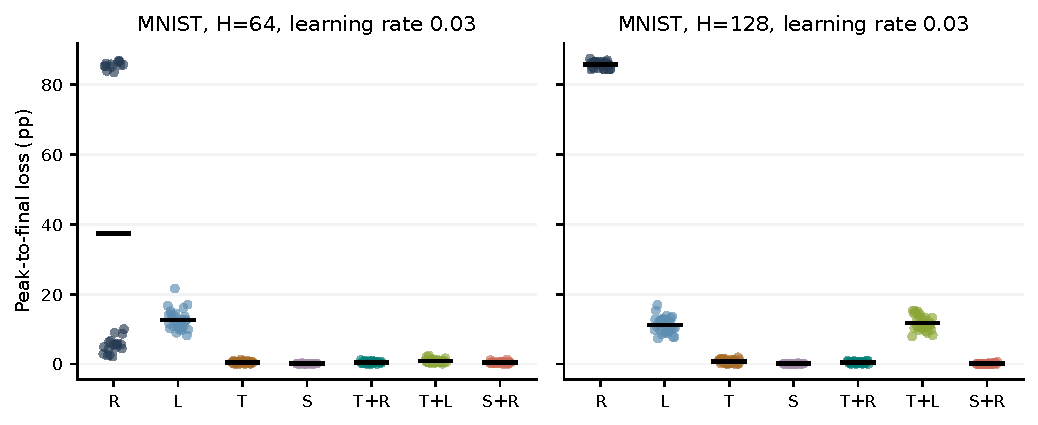
\includegraphics[width=\linewidth]{figures/drop_seeds.pdf}
\caption{Peak-to-final validation loss at learning rate 0.03. Each point is one seed; black marks show the mean. R: ReLU, L: leaky-ReLU, T: tanh, S: sigmoid. Plus signs name fixed mixed pairs. Small losses indicate that the final model keeps its earlier performance.}
\label{fig:drops}\end{figure}

No failures in 30 runs does not mean the failure risk is zero. Under independent seed sampling, the one-sided 95\% upper binomial bound for zero failures out of 30 is about 9.5\%. Also, the selected ReLU checkpoint remains useful in many runs that later fail. The advantage is most direct for training behavior and the final model; it is not an 86-point gain in the best saved test model. At the same LR=0.03, selected-checkpoint test means are 96.071\% for ReLU and 96.766\% for tanh--ReLU, a paired gain of +0.695 pp with 30/30 positive seed differences and a pointwise paired 95\% interval of $[0.612,0.777]$ pp. This fixed-rate result does not replace the tuned-baseline comparison in Section~\ref{sec:tuning}.

\subsection{Width changes the protection}
The six-seed calibration grid extends the width check beyond H=64 and 128 (Table~\ref{tab:widthstability}). At MNIST LR=0.03, ReLU has near-chance final failures at every tested width from 64 to 512: 3/6 at H=64 and 6/6 at H=128, 256, and 512. Tanh--ReLU has no such failures at any tested width. Yet at H=512, all six hybrid runs peak at epochs 2--4 and lose accuracy, ending between 58.30\% and 79.24\%. Their mean final score is 72.843\%, with a mean peak-to-final drop of 22.153 pp. Thus mixing avoids near-chance failure here but does not retain high accuracy.

The same grid gives a sharper limit on CIFAR-10. At LR=0.03, tanh--ReLU has 0--1 final failures out of six at widths up to 128, but 6/6 at both H=256 and 512. These tuning seeds are a useful width check, not an independent confirmation: their results also helped choose the learning rates.

\begin{table}[htbp]
\centering
\caption{CE calibration at LR=0.03: mean final validation accuracy (\%) and final failures below 15\% in parentheses. Each cell has six seeds.}
\label{tab:widthstability}
\footnotesize
\begin{tabular}{@{}llrrrrrr@{}}
\toprule
Data & Model & 12 & 32 & 64 & 128 & 256 & 512 \\
\midrule
MNIST & ReLU & 50.8 (0) & 89.6 (0) & 51.6 (3) & 10.4 (6) & 10.7 (6) & 10.3 (6) \\
MNIST & tanh & 91.9 (0) & 94.8 (0) & 96.3 (0) & 94.8 (0) & 91.4 (0) & 81.8 (0) \\
MNIST & tanh + ReLU & 89.3 (0) & 95.1 (0) & 96.3 (0) & 96.8 (0) & 94.8 (0) & 72.8 (0) \\
CIFAR-10 & ReLU & 10.2 (6) & 11.4 (5) & 12.2 (4) & 11.0 (5) & 10.1 (6) & 10.2 (6) \\
CIFAR-10 & tanh & 25.8 (0) & 22.8 (0) & 21.4 (0) & 13.8 (3) & 10.2 (6) & 10.0 (6) \\
CIFAR-10 & tanh + ReLU & 25.8 (0) & 25.3 (0) & 21.9 (1) & 20.1 (1) & 10.5 (6) & 10.0 (6) \\
\bottomrule
\end{tabular}
\par\smallskip{\footnotesize These are tuning seeds 101--106, used here for an exploratory width check. They are not additional 30-seed tests.}
\end{table}


\subsection{Different loss patterns behind poor final scores}
Figure~\ref{fig:lossdynamics} adds the online training CE traces. On MNIST H=128 at LR=0.03, ReLU's final loss is $2.3081\pm0.0003$ across seeds, close to $\ln(10)=2.3026$, the CE of uniform ten-class probabilities. Together with almost single-class final predictions, this is consistent with a model that has largely lost useful input dependence. It does not prove that the full output vector is constant across inputs or that all units in a hidden layer are inactive.

The ReLU loss minimum occurs at epochs 6--13 (median 9). The first validation score below 15\% follows that minimum by 12.5 epochs on average (range 7--17). This is a look-back summary using the whole curve, not a tested online alarm or a precise estimate of when deterioration first starts. It suggests that loss traces may reveal trouble before accuracy reaches chance level.

Leaky-ReLU shows a different pattern. All 30 runs have their largest one-epoch loss increase at epochs 13--15. For tanh--leaky-ReLU, the corresponding range is 23--26. Mean jump sizes are about 4.57 and 4.46, and final online losses are 3.774 and 4.182 despite final validation accuracy near 85\%. Large loss with useful accuracy is consistent with some very confident errors, but the two logs measure different prediction states and do not establish confidence calibration. In contrast, tanh--ReLU has final online loss 0.0484 and median minimum-loss epoch 38. No delayed failure is seen within 40 epochs; longer runs are needed to test whether this persists.

\begin{figure}[htbp]\centering
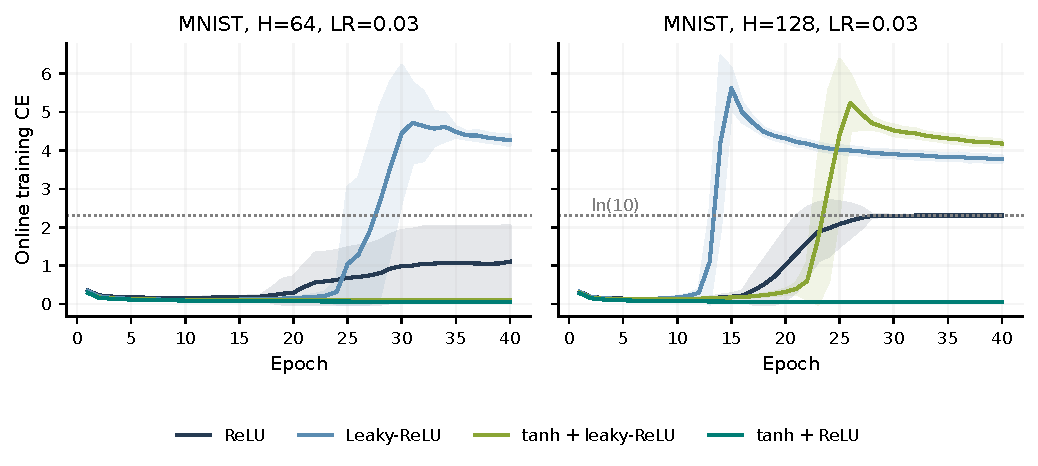
\includegraphics[width=\linewidth]{figures/loss_dynamics.pdf}
\caption{Online training CE at MNIST LR=0.03. Lines are means over 30 seeds; bands are $\pm1$ sample SD. The dotted line is $\ln(10)$. ReLU loses useful performance, while leaky models show a distinct large loss jump. Low hybrid loss lasts through the recorded 40 epochs.}
\label{fig:lossdynamics}\end{figure}
\begin{table}[htbp]
\centering
\caption{MNIST H=128, LR=0.03: online CE loss patterns over 30 seeds. SD is the sample standard deviation.}
\label{tab:losssignatures}
\footnotesize
\begin{tabular}{@{}lrrrr@{}}
\toprule
Model & Final CE, mean $\pm$ SD & Min. epoch (median) & Max. jump epoch & Mean jump \\
\midrule
ReLU & 2.3081 $\pm$ 0.0003 & 6--13 (9) & 17--28 & 1.266 \\
Leaky-ReLU & 3.7739 $\pm$ 0.0862 & 5--9 (7) & 13--15 & 4.570 \\
tanh + leaky-ReLU & 4.1822 $\pm$ 0.0872 & 5--11 (7) & 23--26 & 4.456 \\
tanh + ReLU & 0.0484 $\pm$ 0.0061 & 21--40 (38) & 6--40 & 0.012 \\
\bottomrule
\end{tabular}
\par\smallskip{\footnotesize The largest jump is the maximum consecutive-epoch increase, computed separately for each seed. Its epoch range is meaningful only when the jump is large. Loss is collected while weights change; it is not a fixed-checkpoint validation loss.}
\end{table}


\subsection{The useful range depends on the rule}
Figure~\ref{fig:lrscores} gives the full mean learning-rate curves. At MNIST H=128, the tanh--ReLU range within 1 pp of its own best grid mean is 0.0003--0.02. ReLU's range is 0.0003--0.01. The largest passing rate doubles, while the log span increases from 1.523 to 1.824 decades, about 20\%. At H=64, both models have the same near-best range. We therefore do not assign one general robustness multiplier to the hybrid.

\begin{figure}[htbp]\centering
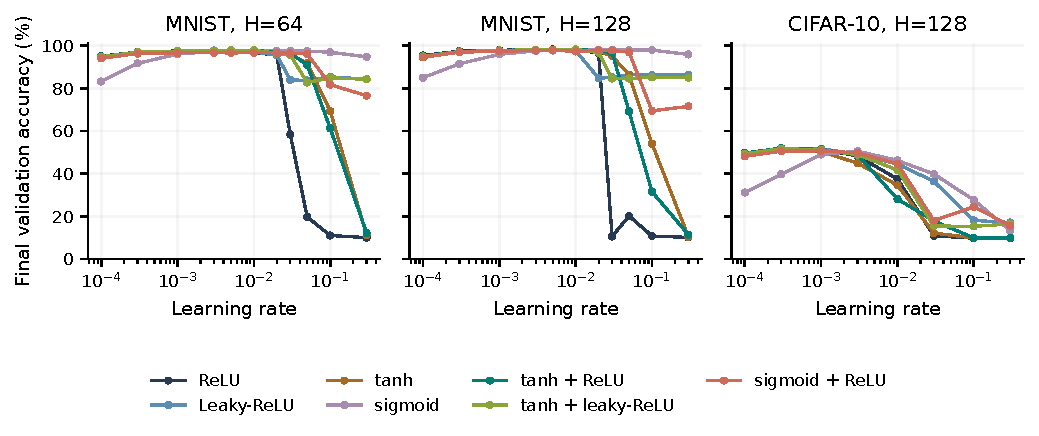
\includegraphics[width=\linewidth]{figures/lr_scores.pdf}
\caption{Mean final validation accuracy over the tested learning rates. Each point contains 30 seeds. Lines connect tested values only; they do not describe untested rates. MNIST uses 11 rates and CIFAR-10 uses eight. Full numerical values are in Appendix~\ref{app:lr}.}
\label{fig:lrscores}\end{figure}

Under the no-final-score-below-15\% rule, the MNIST upper rate rises from 0.02 for ReLU to 0.05 for tanh--ReLU at both widths. That 2.5-fold ratio hides large partial losses. At H=128 and LR=0.05, all 30 hybrid runs lose more than 10 pp; their final mean is 69.273\%, their mean drop is 23.243 pp, and their mean selected epoch is 2.73. Pure tanh and leaky-ReLU both finish near 86.4\% at that rate.

Requiring no run to lose more than 10 pp changes the upper rates to 0.02 for ReLU and 0.03 for tanh--ReLU at both widths, a 1.5-fold ratio. Even this is a ratio of sampled rate limits, not a general robustness factor. At H=64, 3/30 hybrid runs fail this stricter rule at 0.05; at H=128, all 30 do. Leaky-ReLU has large drops in 24/30 H=128 runs already at LR=0.02, where ReLU has none. Tables~\ref{tab:windows} and \ref{tab:dropthreshold} keep these measures separate.

\begin{table}[htbp]
\centering
\caption{Passing learning-rate ranges on the tested grid. Parentheses give the number of sampled rates.}
\label{tab:windows}
\footnotesize
\begin{tabular}{@{}lrlrrr@{}}
\toprule
Data & H & Model & Near best & No final $<15\%$ & No drop $>10$ pp \\
\midrule
MNIST & 64 & R & 0.0003--0.01 (5) & 0.0001--0.02 (7) & 0.0001--0.02 (7) \\
MNIST & 64 & L & 0.001--0.01 (4) & 0.0001--0.3 (11) & 0.0001--0.02 (7) \\
MNIST & 64 & T & 0.0003--0.02 (6) & 0.0001--0.1 (10) & 0.0001--0.05 (9) \\
MNIST & 64 & S & 0.003--0.1 (7) & 0.0001--0.3 (11) & 0.0001--0.3 (11) \\
MNIST & 64 & T+R & 0.0003--0.01 (5) & 0.0001--0.05 (9) & 0.0001--0.03 (8) \\
MNIST & 64 & T+L & 0.0003--0.01 (5) & 0.0001--0.3 (11) & 0.0001--0.03 (8) \\
MNIST & 64 & S+R & 0.0003--0.05 (8) & 0.0001--0.1 (10) & 0.0001--0.05 (9) \\
MNIST & 128 & R & 0.0003--0.01 (5) & 0.0001--0.02 (7) & 0.0001--0.02 (7) \\
MNIST & 128 & L & 0.0003--0.01 (5) & 0.0001--0.3 (11) & 0.0001--0.01 (6) \\
MNIST & 128 & T & 0.001--0.02 (5) & 0.0001--0.1 (10) & 0.0001--0.03 (8) \\
MNIST & 128 & S & 0.003--0.1 (7) & 0.0001--0.3 (11) & 0.0001--0.3 (11) \\
MNIST & 128 & T+R & 0.0003--0.02 (6) & 0.0001--0.05 (9) & 0.0001--0.03 (8) \\
MNIST & 128 & T+L & 0.001--0.01 (4) & 0.0001--0.3 (11) & 0.0001--0.02 (7) \\
MNIST & 128 & S+R & 0.0003--0.05 (8) & 0.0001--0.1 (10) & 0.0001--0.05 (9) \\
CIFAR-10 & 128 & R & 0.0003--0.001 (2) & 0.0001--0.01 (5) & 0.0001--0.3 (8) \\
CIFAR-10 & 128 & L & 0.0003--0.001 (2) & 0.0001--0.03 (6) & 0.0001--0.003 (4) \\
CIFAR-10 & 128 & T & 0.0003--0.001 (2) & 0.0001--0.01 (5) & 0.0001--0.01 (5) \\
CIFAR-10 & 128 & S & 0.003--0.003 (1) & 0.0001--0.1 (7) & 0.0001--0.3 (8) \\
CIFAR-10 & 128 & T+R & 0.0003--0.001 (2) & 0.0001--0.003 (4) & 0.0001--0.003 (4) \\
CIFAR-10 & 128 & T+L & 0.0003--0.001 (2) & 0.0001--0.01 (5) & 0.0001--0.01 (5) \\
CIFAR-10 & 128 & S+R & 0.0003--0.001 (2) & 0.0001--0.01 (5) & 0.0001--0.01 (5) \\
\bottomrule
\end{tabular}
\par\smallskip{\footnotesize Near best: mean final score within 1 pp of the model's own best grid mean. Each no-event rule requires all 30 seeds to pass. Ranges are the widest consecutive passing sets, chosen by log span; untested rates are unknown. Small drops alone do not imply high accuracy. Model codes follow Figure~\ref{fig:drops}.}
\end{table}

\begin{table}[htbp]
\centering
\caption{MNIST runs losing more than 10 pp from peak to final validation accuracy.}
\label{tab:dropthreshold}
\small
\begin{tabular}{@{}rlrrrr@{}}
\toprule
H & Model & LR=0.02 & 0.03 & 0.05 & 0.1 \\
\midrule
64 & ReLU & 0/30 & 12/30 & 30/30 & 11/30 \\
64 & tanh & 0/30 & 0/30 & 0/30 & 11/30 \\
64 & Leaky-ReLU & 0/30 & 25/30 & 13/30 & 0/30 \\
64 & tanh + ReLU & 0/30 & 0/30 & 3/30 & 12/30 \\
128 & ReLU & 0/30 & 30/30 & 30/30 & 20/30 \\
128 & tanh & 0/30 & 0/30 & 1/30 & 14/30 \\
128 & Leaky-ReLU & 24/30 & 19/30 & 1/30 & 0/30 \\
128 & tanh + ReLU & 0/30 & 0/30 & 30/30 & 18/30 \\
\bottomrule
\end{tabular}
\par\smallskip{\footnotesize A zero count does not ensure a high score: a run that never learns can also have a small drop.}
\end{table}


\subsection{Higher rates can reflect a shift of the curve}
At both MNIST widths, the largest mean final validation score occurs at LR=0.005 for ReLU and 0.01 for tanh--ReLU. Thus LR=0.03 is six times ReLU's own best sampled rate but only three times the hybrid's. Figure~\ref{fig:normalizedlr} divides the horizontal axis by each model's own best sampled rate and subtracts its best mean score on the vertical axis. These are descriptive summaries of the same evaluation grid, not new tuning choices used to select test results.

Starting from that best rate and moving upward along consecutive grid points, the final score stays within 5 pp through LR=0.02 for ReLU and 0.03 for tanh--ReLU. The ratios to the respective best rates are 4 and 3. This measure gives no wider upper range to the hybrid after scaling. Pure sigmoid at H=128 stays within 5 pp through LR=0.3, ten times its best sampled rate of 0.03. The modest near-best span gain at H=128 remains real under the 1-pp rule, but the full picture supports a rightward shift more clearly than a general widening. Different grids and longer runs are needed to separate these effects more firmly.

\begin{figure}[htbp]\centering
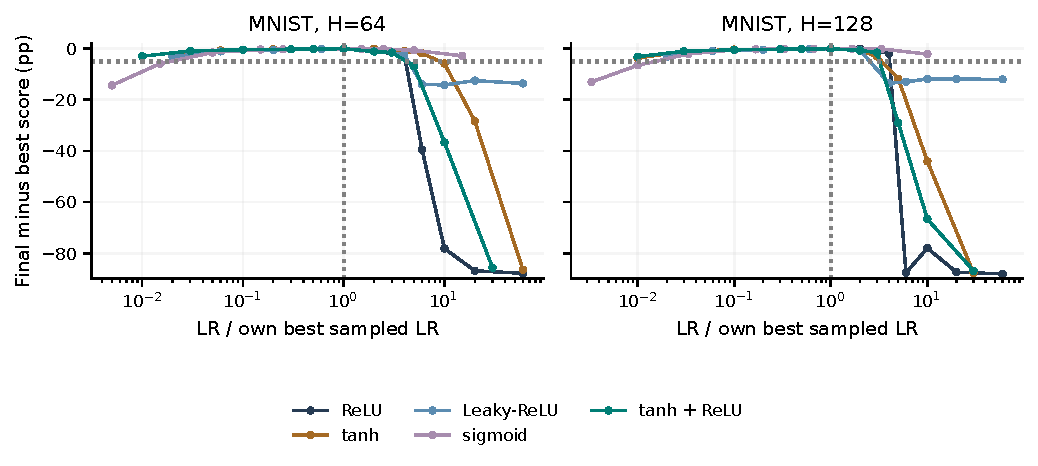
\includegraphics[width=\linewidth]{figures/normalized_lr.pdf}
\caption{MNIST learning-rate curves relative to each model's own best sampled mean final score. Vertical lines mark the best rate; horizontal lines mark a 5-pp loss from the best score. Each point uses 30 seeds. Normalization exposes a shift in useful rate as well as any change in range; it does not hold effective update size fixed.}
\label{fig:normalizedlr}\end{figure}

\subsection{The benefit does not transfer in full to CIFAR-10}
At CIFAR-10 H=128 and learning rate 0.03, tanh--ReLU has fewer final near-chance failures than ReLU: 9/30 versus 26/30. Yet its final validation mean is only 17.879\%, far below its low-rate scores. Leaky-ReLU keeps 36.411\% and has no near-chance failures at that rate. At learning rate 0.01, tanh--ReLU is worse than both controls, with mean 28.110\% and one failure. Table~\ref{tab:cifarstress} shows these cases.

\begin{table}[htbp]
\centering
\caption{CIFAR-10, H=128. Leaky-ReLU is an important control. Each row has 30 seeds.}
\label{tab:cifarstress}
\small
\begin{tabular}{@{}llrrrr@{}}
\toprule
LR & Model & Final acc. (\%) & Peak acc. (\%) & Loss (pp) & Below 15\% \\
\midrule
0.0003 & ReLU & 51.887 & 52.753 & 0.867 & 0/30 \\
0.0003 & tanh + ReLU & 52.006 & 52.744 & 0.738 & 0/30 \\
0.0003 & Leaky-ReLU & 51.709 & 52.541 & 0.831 & 0/30 \\
0.003 & ReLU & 48.351 & 49.786 & 1.435 & 0/30 \\
0.003 & tanh + ReLU & 48.833 & 49.981 & 1.148 & 0/30 \\
0.003 & Leaky-ReLU & 49.223 & 50.867 & 1.644 & 0/30 \\
0.01 & ReLU & 37.516 & 40.855 & 3.339 & 0/30 \\
0.01 & tanh + ReLU & 28.110 & 37.652 & 9.542 & 1/30 \\
0.01 & Leaky-ReLU & 44.602 & 47.206 & 2.604 & 0/30 \\
0.03 & ReLU & 10.903 & 15.503 & 4.600 & 26/30 \\
0.03 & tanh + ReLU & 17.879 & 26.346 & 8.467 & 9/30 \\
0.03 & Leaky-ReLU & 36.411 & 41.501 & 5.090 & 0/30 \\
\bottomrule
\end{tabular}
\end{table}


The time course differs from MNIST (Figure~\ref{fig:cifardynamics}). At CIFAR-10 LR=0.03, 29/30 ReLU runs are below 15\% after the first epoch, and all 30 are below it at least once. Their mean per-run peak is only 15.503\%. This is mainly failure to learn useful accuracy, rather than late loss after strong learning. The hybrid reaches a mean per-run peak of 26.346\%, but 18/30 runs fall below 15\% at least once, compared with 9/30 at the final epoch. The endpoint rule therefore misses some poor intermediate states.

At LR=0.01, ReLU and tanh select late epochs (median 34.5 and 34), while the hybrid selects a median epoch of 12 and falls to 28.110\%. Its mean accuracy curve peaks at 35.786\%; this differs from the mean of each run's peak, 37.652\%. The six-seed calibration grid also places tanh--ReLU below both parents at widths 32, 64, 128, and 256 at this rate. Mixing can therefore create a poorer trajectory even when each parent retains a better final score.

\begin{figure}[htbp]\centering
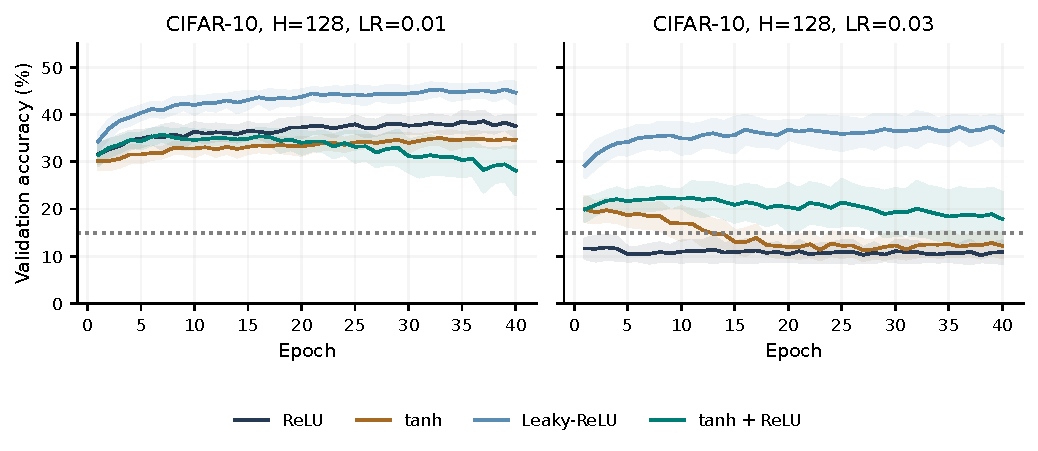
\includegraphics[width=\linewidth]{figures/cifar_dynamics.pdf}
\caption{CIFAR-10 H=128 validation curves. Lines and bands show means and $\pm1$ seed SD over 30 runs. ReLU learns little at LR=0.03; at LR=0.01, the hybrid loses accuracy while its parents improve. The dotted line marks 15\%.}
\label{fig:cifardynamics}\end{figure}
\begin{table}[htbp]
\centering
\caption{CIFAR-10 H=128: final failure and failure at any logged epoch are distinct measures. Each row has 30 seeds.}
\label{tab:cifaronset}
\footnotesize
\begin{tabular}{@{}llrrrr@{}}
\toprule
LR & Model & Epoch 1 $<15\%$ & Any epoch $<15\%$ & Final $<15\%$ & Median best epoch \\
\midrule
0.01 & ReLU & 0 & 0 & 0 & 34.5 \\
0.01 & tanh & 0 & 0 & 0 & 34 \\
0.01 & Leaky-ReLU & 0 & 0 & 0 & 36 \\
0.01 & tanh + ReLU & 0 & 1 & 1 & 12 \\
0.03 & ReLU & 29 & 30 & 26 & 9 \\
0.03 & tanh & 1 & 30 & 27 & 4.5 \\
0.03 & Leaky-ReLU & 0 & 0 & 0 & 28.5 \\
0.03 & tanh + ReLU & 1 & 18 & 9 & 20 \\
\bottomrule
\end{tabular}
\end{table}


The near-best grid range is the same for ReLU and tanh--ReLU on CIFAR-10: 0.0003--0.001. Under the consecutive no-failure rule, the mixed model's range ends earlier because of its failure at 0.01. These results rule out a dataset-wide or function-pair-wide claim that mixing always improves stability. Figure~\ref{fig:failmaps} includes all failures in the evaluation grids.

\begin{figure}[htbp]\centering
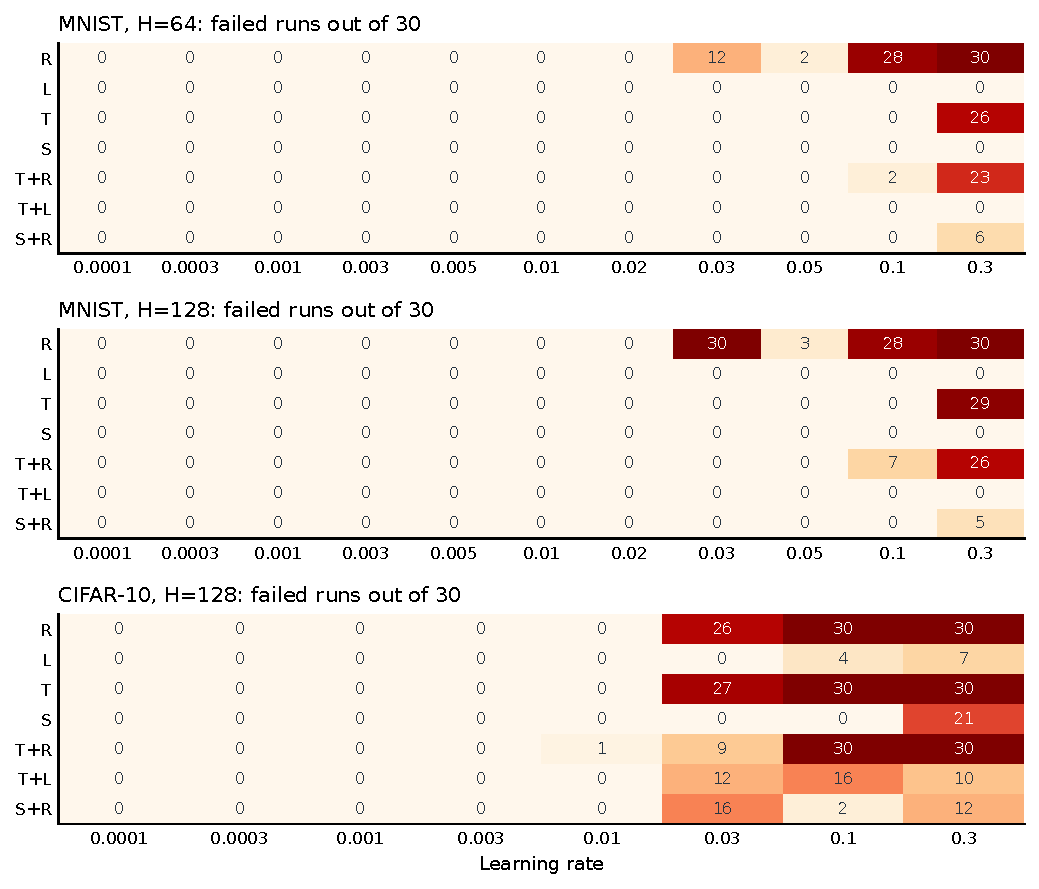
\includegraphics[width=0.94\linewidth]{figures/failure_maps.pdf}
\caption{Number of runs, out of 30, ending below 15\% validation accuracy. The lightest cells mean zero observed failures. The full grid shows that lower failure risk at one rate does not imply a wider failure-free range across all rates. Model codes follow Figure~\ref{fig:drops}.}
\label{fig:failmaps}\end{figure}

\FloatBarrier
\section{Test accuracy and other benefits}
\subsection{Width and activation choice}
Tables~\ref{tab:mnist:test_acc_best} and \ref{tab:cifar10:test_acc_best} show all main-grid accuracy means and SDs. The tests retain the original tuning choices. The largest MNIST mean is 98.289\% for tanh--ReLU at H=512, compared with 98.285\% for ReLU. CIFAR-10 has its largest mean with ReLU at H=512, 54.875\%, compared with 54.711\% for tanh--ReLU. These are observed ranks, not clear evidence of distinct best models.

\begin{table}[htbp]
\centering
\caption{MNIST checkpoint test accuracy (\%). Mean $\pm$ seed SD, $n=30$.}
\label{tab:mnist:test_acc_best}
\footnotesize
\begin{tabular}{@{}lrrrrrr@{}}
\toprule
Model & 12 & 32 & 64 & 128 & 256 & 512 \\
\midrule
ReLU & 94.30 $\pm$ 0.30 & 96.71 $\pm$ 0.19 & 97.58 $\pm$ 0.13 & 97.86 $\pm$ 0.07 & 98.21 $\pm$ 0.07 & 98.29 $\pm$ 0.06 \\
Leaky-ReLU & 94.27 $\pm$ 0.23 & 96.68 $\pm$ 0.19 & 97.56 $\pm$ 0.11 & 97.85 $\pm$ 0.08 & 98.18 $\pm$ 0.06 & 98.25 $\pm$ 0.09 \\
tanh & 93.95 $\pm$ 0.26 & 96.37 $\pm$ 0.16 & 97.39 $\pm$ 0.12 & 97.83 $\pm$ 0.09 & 98.02 $\pm$ 0.07 & 98.02 $\pm$ 0.07 \\
sigmoid & 93.77 $\pm$ 0.33 & 96.27 $\pm$ 0.14 & 97.12 $\pm$ 0.08 & 97.66 $\pm$ 0.09 & 97.97 $\pm$ 0.07 & 98.04 $\pm$ 0.07 \\
tanh + ReLU & 93.99 $\pm$ 0.25 & 96.52 $\pm$ 0.18 & 97.58 $\pm$ 0.13 & 98.04 $\pm$ 0.07 & 98.21 $\pm$ 0.07 & 98.29 $\pm$ 0.09 \\
tanh + leaky-ReLU & 94.02 $\pm$ 0.32 & 96.51 $\pm$ 0.16 & 97.61 $\pm$ 0.12 & 97.99 $\pm$ 0.08 & 98.19 $\pm$ 0.07 & 98.27 $\pm$ 0.08 \\
sigmoid + ReLU & 93.77 $\pm$ 0.39 & 95.99 $\pm$ 0.17 & 96.71 $\pm$ 0.16 & 97.55 $\pm$ 0.14 & 98.04 $\pm$ 0.08 & 98.12 $\pm$ 0.07 \\
\bottomrule
\end{tabular}
\par\smallskip{\footnotesize Main hybrids use a 50:50 split. These cells keep the original learning-rate choices.}
\end{table}

\begin{table}[htbp]
\centering
\caption{CIFAR-10 checkpoint test accuracy (\%). Mean $\pm$ seed SD, $n=30$.}
\label{tab:cifar10:test_acc_best}
\footnotesize
\begin{tabular}{@{}lrrrrrr@{}}
\toprule
Model & 12 & 32 & 64 & 128 & 256 & 512 \\
\midrule
ReLU & 43.46 $\pm$ 0.74 & 49.19 $\pm$ 0.59 & 51.24 $\pm$ 0.50 & 53.04 $\pm$ 0.53 & 54.07 $\pm$ 0.51 & 54.88 $\pm$ 0.47 \\
Leaky-ReLU & 43.62 $\pm$ 0.88 & 49.25 $\pm$ 0.49 & 51.27 $\pm$ 0.49 & 52.95 $\pm$ 0.51 & 53.85 $\pm$ 0.48 & 54.61 $\pm$ 0.42 \\
tanh & 42.34 $\pm$ 0.56 & 47.89 $\pm$ 0.48 & 50.49 $\pm$ 0.39 & 51.93 $\pm$ 0.52 & 52.49 $\pm$ 0.50 & 53.19 $\pm$ 0.49 \\
sigmoid & 41.36 $\pm$ 0.38 & 47.21 $\pm$ 0.55 & 50.01 $\pm$ 0.36 & 51.66 $\pm$ 0.46 & 52.78 $\pm$ 0.53 & 53.14 $\pm$ 0.53 \\
tanh + ReLU & 42.91 $\pm$ 0.65 & 48.80 $\pm$ 0.45 & 51.60 $\pm$ 0.38 & 53.22 $\pm$ 0.44 & 54.23 $\pm$ 0.46 & 54.71 $\pm$ 0.43 \\
tanh + leaky-ReLU & 42.99 $\pm$ 0.76 & 48.76 $\pm$ 0.45 & 51.29 $\pm$ 0.44 & 53.09 $\pm$ 0.52 & 53.98 $\pm$ 0.40 & 54.47 $\pm$ 0.37 \\
sigmoid + ReLU & 42.34 $\pm$ 0.86 & 47.77 $\pm$ 0.61 & 50.27 $\pm$ 0.43 & 51.90 $\pm$ 0.45 & 53.48 $\pm$ 0.50 & 54.36 $\pm$ 0.51 \\
\bottomrule
\end{tabular}
\par\smallskip{\footnotesize Main hybrids use a 50:50 split. These cells keep the original learning-rate choices.}
\end{table}


Figure~\ref{fig:width} shows both accuracy and macro-F1. Their trends mostly agree. Mixed activations can match the stronger parent without adding weights, but mixing by itself is not enough to improve a model. Sigmoid--ReLU scores below ReLU at all main widths on both datasets. At small widths, giving each function fewer neurons may limit learning, but we have no feature-level measurements to establish this cause.

\begin{figure}[htbp]\centering
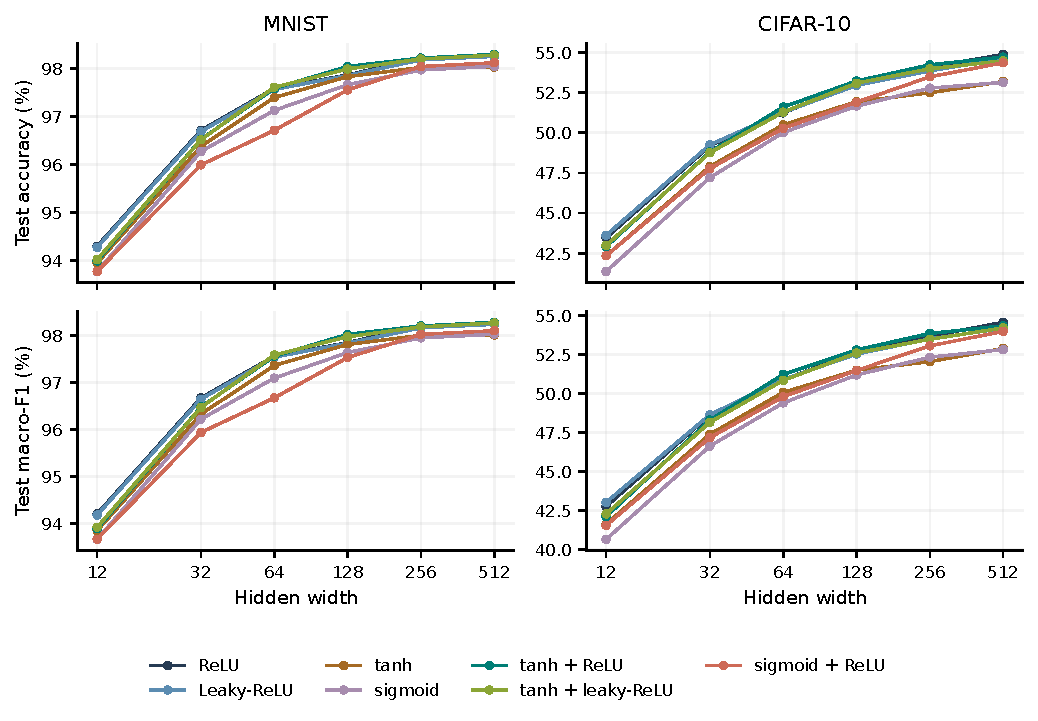
\includegraphics[width=\linewidth]{figures/width_scores.pdf}
\caption{Checkpoint accuracy and macro-F1 across width. Each point is a mean over 30 seeds. All seven models share the same parameter count at a given width. Error estimates for accuracy are in the main tables; F1 means and SDs are in Appendix~\ref{app:main}.}
\label{fig:width}\end{figure}

The paired tanh--ReLU effects change with width (Figure~\ref{fig:paired}). On MNIST the model is worse at H=12 and 32, close at H=64, apparently better at H=128 under the original tuning rule, and close again at H=256 and 512. There is no steady increase in benefit as width grows. The CIFAR-10 H=64 difference is +0.363 pp, but its adjusted p-value is 0.095 across the 120 main tests. Full paired values appear in Appendix~\ref{app:main}.

\begin{figure}[htbp]\centering
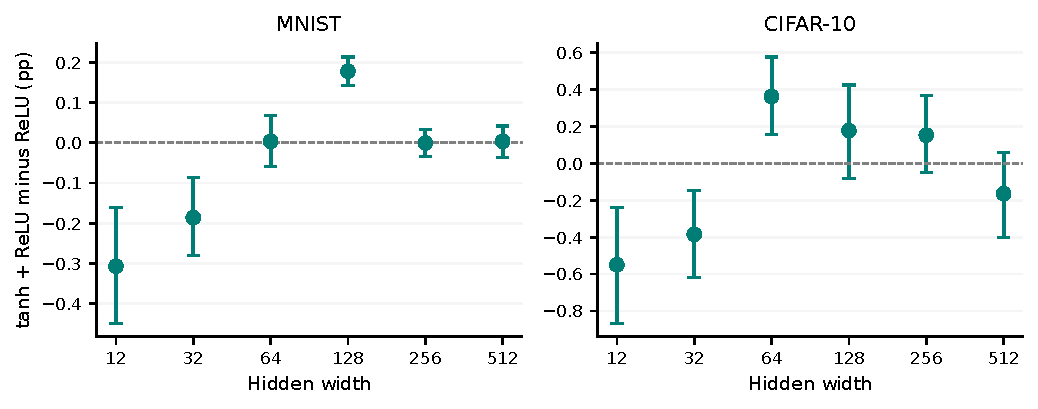
\includegraphics[width=\linewidth]{figures/paired_width.pdf}
\caption{Paired test-accuracy differences using the original learning rates. Bars are pointwise 95\% bootstrap intervals, not seed SDs. The MNIST H=128 result is sensitive to the baseline learning rate; Table~\ref{tab:aligned} gives the matched selection check.}
\label{fig:paired}\end{figure}

\subsection{The tuning target matters}\label{sec:tuning}
The original learning-rate rule uses final validation accuracy, while the test model is selected by peak validation accuracy. Changing tuning to mean peak validation accuracy changes 17 of 84 main choices. Existing evaluation grids cover four of these changes. The remaining thirteen need further runs for a fully retuned main comparison. We keep this distinction clear rather than filling missing cells from test scores.

The most important check is MNIST H=128. ReLU tuning changes from 0.003 to 0.01, while tanh--ReLU stays at 0.01. Its test gain falls from +0.178 pp to +0.029 pp (Table~\ref{tab:aligned}). The latter paired interval includes zero and the paired t-test gives $p=0.266$. Relative error reduction falls from 8.30\% to about 1.47\%. About 83.5\% of the original mean difference is removed by this change. The selection check uses validation data from separate tuning seeds, not a search for the highest evaluation test score.

\begin{table}[htbp]
\centering
\caption{MNIST, H=128: aligning the ReLU learning rate with checkpoint selection. The hybrid uses LR=0.01 in both rows.}
\label{tab:aligned}
\small
\begin{tabular}{@{}rrrrr@{}}
\toprule
ReLU LR & ReLU acc. (\%) & Hybrid acc. (\%) & Difference (pp) & 95\% paired interval \\
\midrule
0.003 & 97.860 & 98.038 & +0.178 & [+0.143, +0.213] \\
0.01 & 98.009 & 98.038 & +0.029 & [-0.017, +0.080] \\
\bottomrule
\end{tabular}
\end{table}


This check does not remove the fixed-rate stability result at 0.03. It changes a different claim: whether mixing gives better best-checkpoint test accuracy after tuning. Treating those claims separately prevents a training-failure control from overstating the value of a model that can be tuned to work well.

\subsection{Activation share and layout}
At MNIST H=128, the ratio tests assign 32, 64, or 96 neurons per hidden layer to the second function. All tests use interleave layout and LR=0.01. The parameter count is 118,282 for every ratio. Table~\ref{tab:ratios} gives their results.

\begin{table}[htbp]
\centering
\caption{Allocation ratio at MNIST H=128 and LR=0.01. The second function is ReLU or leaky-ReLU. Each row has 30 seeds.}
\label{tab:ratios}
\footnotesize
\begin{tabular}{@{}lrrrr@{}}
\toprule
Model & $\rho$ & Accuracy (\%), mean $\pm$ SD & Macro-F1 (\%) & Selected epoch \\
\midrule
tanh + ReLU & 0.25 & 97.957 $\pm$ 0.099 & 97.937 & 19.8 \\
tanh + ReLU & 0.50 & 98.038 $\pm$ 0.073 & 98.020 & 24.0 \\
tanh + ReLU & 0.75 & 98.052 $\pm$ 0.079 & 98.036 & 23.6 \\
tanh + leaky-ReLU & 0.25 & 97.965 $\pm$ 0.096 & 97.944 & 21.6 \\
tanh + leaky-ReLU & 0.50 & 97.986 $\pm$ 0.081 & 97.967 & 21.2 \\
tanh + leaky-ReLU & 0.75 & 98.052 $\pm$ 0.084 & 98.035 & 25.0 \\
\bottomrule
\end{tabular}
\end{table}


Increasing the ReLU share from 25\% to 50\% raises mean test accuracy by 0.081 pp. Moving from 50\% to 75\% adds only 0.014 pp, with a paired interval that includes zero. For the tanh--leaky-ReLU pair, the 50\% to 75\% change adds 0.066 pp and has an adjusted p-value of 0.015 within the six ratio tests. Both 75\% models reach the same mean accuracy, 98.052\%. Figure~\ref{fig:ratio} includes pure-function controls at the same learning rate.

\begin{figure}[htbp]\centering
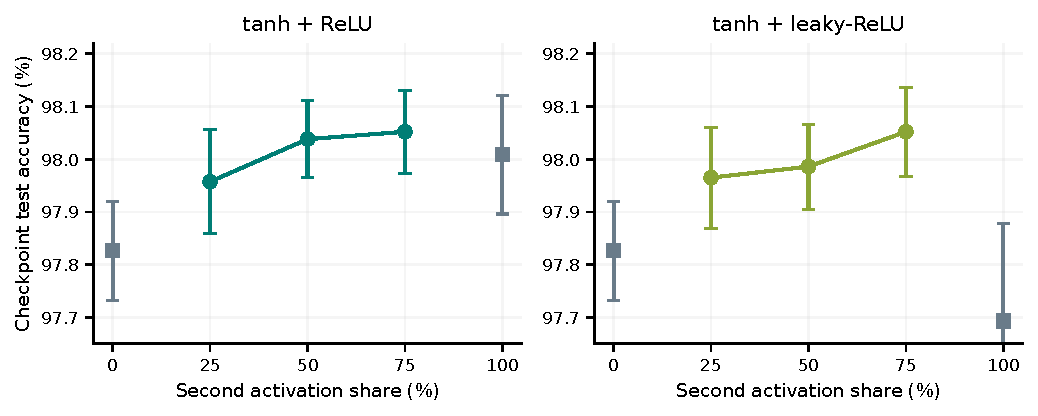
\includegraphics[width=\linewidth]{figures/ratio_scores.pdf}
\caption{Activation share at MNIST H=128 and LR=0.01. Circles are the ratio tests; squares are single-function controls from the learning-rate sweep. Bars show seed SD. For tanh--ReLU, 75\% gives 98.052\% and pure ReLU gives 98.009\%; their paired difference is not clearly above zero. These are accuracy tests at one LR, not high-rate stability tests of the other ratios.}
\label{fig:ratio}\end{figure}

At the common LR=0.01, pure ReLU reaches 98.009\%. The 75\% tanh--ReLU model is +0.043 pp higher, with a paired interval of about $[-0.005,+0.093]$. Thus the ratio results do not identify a universal best split. In particular, we cannot claim that a 75\% ReLU layer keeps the 50\% layer's stability at LR=0.03: no such ratio-by-rate test was run. Ratios also did not receive separate LR tuning.

Block and random layouts give small differences from interleave (Appendix~\ref{app:ratio}). In a fully connected network, a neuron permutation with matching weight permutations leaves the model's function unchanged. Also, making the random mask uses random numbers that later affect weights and training order. Same seed labels therefore do not hold all these factors fixed in the random-layout comparison. The tests do not establish a special advantage of neuron position.

\subsection{Loss function and output layer}
The MSE runs do not show a stable gain for tanh--ReLU over ReLU (Table~\ref{tab:mse}). At H=64, the difference is $-0.202$ pp, with a paired interval of about $[-0.265,-0.138]$. At H=128, it is $-0.034$ pp and the interval includes zero. The H=64 mixed model's tuning choice also changes under the peak rule, but matching evaluation runs are not available.

\begin{table}[htbp]
\centering
\caption{MNIST with the implemented MSE loss and sigmoid output. Mean and SD use 30 seeds. Differences are against ReLU at the same width.}
\label{tab:mse}
\footnotesize
\begin{tabular}{@{}rllrrrr@{}}
\toprule
H & Model & LR & Accuracy (\%) & F1 (\%) & $\Delta$ (pp) & 95\% interval \\
\midrule
64 & ReLU & 0.01 & 97.637 $\pm$ 0.133 & 97.612 & +0.000 & [+0.000, +0.000] \\
64 & tanh & 0.01 & 97.266 $\pm$ 0.132 & 97.232 & -0.371 & [-0.436, -0.311] \\
64 & tanh + ReLU & 0.01 & 97.435 $\pm$ 0.119 & 97.407 & -0.202 & [-0.265, -0.138] \\
128 & ReLU & 0.01 & 97.998 $\pm$ 0.080 & 97.981 & +0.000 & [+0.000, +0.000] \\
128 & tanh & 0.01 & 97.777 $\pm$ 0.070 & 97.752 & -0.221 & [-0.263, -0.177] \\
128 & tanh + ReLU & 0.03 & 97.964 $\pm$ 0.088 & 97.943 & -0.034 & [-0.075, +0.008] \\
\bottomrule
\end{tabular}
\end{table}


The loss/output pair also changes the failure threshold in the six-seed calibration data (Table~\ref{tab:msestability}). At H=128 and LR=0.03, ReLU ends at about 97.9\% with MSE and sigmoid outputs, compared with 10.4\% for CE and softmax on the same tuning seeds. At LR=0.1, ReLU is near chance, but the hybrid also loses much of its accuracy: 75.6\% at H=64 and 36.3\% at H=128. Pure tanh retains 93.9\% and 92.7\%. These observations limit any explanation based only on hidden activation choice.
\begin{table}[htbp]
\centering
\caption{MNIST MSE calibration: mean final validation accuracy (\%) and final failure counts below 15\%. Each cell has six tuning seeds.}
\label{tab:msestability}
\small
\begin{tabular}{@{}rlrr@{}}
\toprule
H & Model & LR=0.03 & LR=0.1 \\
\midrule
64 & ReLU & 93.047 (0/6) & 9.270 (6/6) \\
64 & tanh & 97.383 (0/6) & 93.930 (0/6) \\
64 & tanh + ReLU & 97.683 (0/6) & 75.560 (1/6) \\
128 & ReLU & 97.903 (0/6) & 10.633 (6/6) \\
128 & tanh & 97.973 (0/6) & 92.687 (0/6) \\
128 & tanh + ReLU & 98.257 (0/6) & 36.323 (3/6) \\
\bottomrule
\end{tabular}
\par\smallskip{\footnotesize These runs use sigmoid outputs and the implemented MSE derivative scale. They do not isolate loss choice from output activation or update scale.}
\end{table}


These runs change both the loss and the output activation. There is also an implementation detail: the logged MSE is $\frac{1}{10}\sum_j(o_j-y_j)^2$, while the supplied output derivative is $2(o_j-y_j)$ rather than $\frac{2}{10}(o_j-y_j)$. Updates are therefore ten times the derivative scale of the logged loss before later clipping. We report the completed runs as implemented. They do not isolate the effect of a normalized MSE loss at the same numerical learning rate.

\subsection{Model size and recorded cost}
Mixed masks add no trainable weights at a fixed width. With biases included, the parameter count is
\begin{equation}P(H,D)=H^2+(D+12)H+10.\end{equation}
The choice can therefore improve final training behavior without increasing this count. It does not follow that tanh has the same computation cost as ReLU.

\begin{table}[htbp]
\centering
\caption{Accuracy and size at selected operating points. Seconds are full-run elapsed time under the logged shared workload, not inference time.}
\label{tab:cost}
\small
\begin{tabular}{@{}lrlrrr@{}}
\toprule
Data & H & Model & Accuracy (\%) & Parameters & Seconds \\
\midrule
MNIST & 128 & tanh + ReLU & 98.038 & 118,282 & 219.9 \\
MNIST & 256 & ReLU & 98.214 & 269,322 & 482.5 \\
MNIST & 512 & ReLU & 98.285 & 669,706 & 1456.7 \\
MNIST & 512 & tanh + ReLU & 98.289 & 669,706 & 1474.4 \\
CIFAR-10 & 128 & tanh + ReLU & 53.221 & 411,146 & 761.3 \\
CIFAR-10 & 256 & ReLU & 54.074 & 855,050 & 2240.3 \\
CIFAR-10 & 512 & ReLU & 54.875 & 1,841,162 & 8400.7 \\
CIFAR-10 & 512 & tanh + ReLU & 54.711 & 1,841,162 & 8300.5 \\
\bottomrule
\end{tabular}
\end{table}


Figure~\ref{fig:cost} and Table~\ref{tab:cost} show the width trade-off. MNIST ReLU at H=256 scores 98.214\%, only 0.074 pp below the H=512 tanh--ReLU mean, with 59.8\% fewer parameters and 67.3\% less recorded run time. This saving is mainly a width effect and should not be credited to mixing. On CIFAR-10, ReLU at H=256 gives up 0.802 pp relative to H=512 while using 53.6\% fewer parameters.

\begin{figure}[htbp]\centering
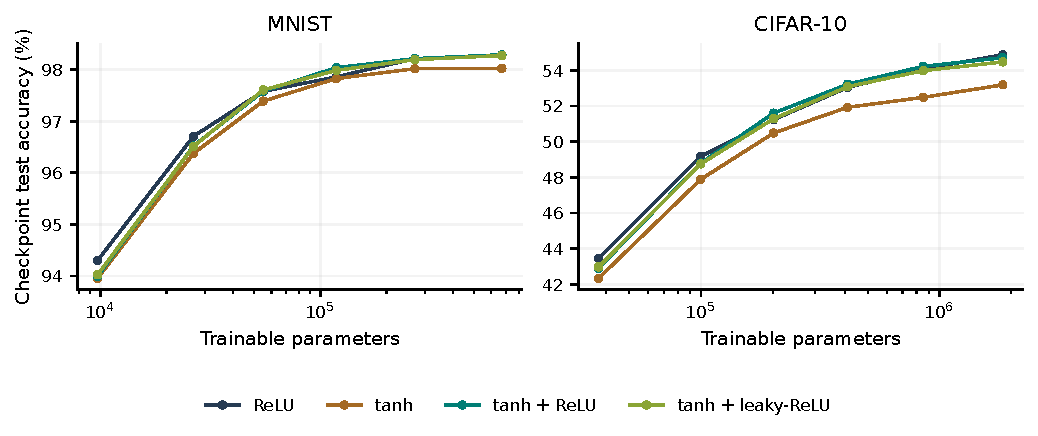
\includegraphics[width=\linewidth]{figures/parameter_cost.pdf}
\caption{Accuracy against parameter count for selected models. Increasing width has a large cost and a shrinking accuracy gain. Mixed and single-function models have equal counts at the same width. The figure does not measure inference latency or energy.}
\label{fig:cost}\end{figure}

Run time includes loading data, training, validation, clean training checks, and final tests. Logs report up to 190 workers on a 192-core ARM system. We do not have isolated timing or energy data. The recorded times can guide further tests but do not establish a deployment speed advantage.

\FloatBarrier
\section{What may explain the stability gain?}
Tanh has bounded outputs, while ReLU keeps a positive linear path. A mixed layer could limit some large signals while retaining paths that do not flatten for positive inputs. The fact that pure tanh remains stable but scores below tanh--ReLU at MNIST LR=0.03 is consistent with this idea. It is not proof of it. Learned weights can still amplify bounded inputs, and half of the neurons still use ReLU.

Leaky-ReLU keeps a gradient on the negative side, which may help avoid a network stuck with inactive units. Its MNIST results show that avoiding chance-level failure can still leave a large loss of accuracy. This is why both the failure count and the peak-to-final loss are useful.

The gradient clip also has limits. If $g$ is the loss derivative with respect to a neuron's weighted input, an update includes the term
\begin{equation}\Delta w=-\eta\,\operatorname{clip}(g,-10,10)\,h.\end{equation}
Large previous-layer output $h$ can still give a large weight step. The fixed initialization scale may also interact with each activation. The loss and prediction traces narrow the hypotheses. A dead ReLU layer is consistent with the near-chance CE and nearly constant predicted label. The large leaky-model loss jumps suggest a different process, such as growth in weight or signal size. Their narrow timing range across seeds makes this worth testing, but does not establish deterministic drift. Activation traces, gradient and weight norms, and clip counts are needed to test these explanations.

Tanh has no zero-gradient negative half-line like ReLU, but this does not guarantee a useful input-dependent path. Tanh can saturate, its output is exactly zero at zero input, and downstream weights can erase its signal. The observed hybrid protection is therefore an empirical finding, not a mathematical guarantee.

Width can also change update size. For one linear output and fixed hidden vector $h$, its SGD update changes the score on that same vector by $\Delta z=-\eta\,\operatorname{clip}(g,-10,10)(\|h\|^2+1)$, including the bias. If per-unit squared outputs stay comparable as width grows, this term grows with width. The actual network also updates hidden layers, so this relation is only a possible route to width-dependent failure, not a measured scaling law. Finally, activation derivatives and the loss/output pair change effective step sizes. The normalized LR curves and MSE check show why a higher nominal rate alone cannot identify the mechanism.

\section{Limits and next tests}
The strongest result is tied to a small MLP, single-example SGD, the implemented initialization, and selected MNIST rates. We have not tested other optimizers, batch sizes, convolutional models, or input attacks. CIFAR-10 already shows that the same benefit need not transfer. The available ratio tests cannot show which share is most stable at high rates.

All seed runs share one split. Their intervals measure training variation on that split, not uncertainty across new datasets. Six tuning seeds may also give unstable learning-rate choices. Many settings were examined before the main result was selected, so the stability analysis is exploratory. The reported correction groups do not remove all selection effects. A fresh set of seeds and splits is needed for an independent check.

The epoch budget may limit some models. On CIFAR-10, 239 of 1,260 main runs choose epoch 40. Larger models also show a growing train--test gap. ReLU's selected-checkpoint gap rises from 1.609 pp at H=12 to 14.318 pp at H=512. The clean training score uses a fixed 10,000-image subset. Appendix~\ref{app:classes} shows these gaps and class-level recall. Longer runs and weight decay would help separate incomplete learning from poor generalization.

Source details were checked against the local runner and layer code, but the logged AWS binary was not rebuilt and matched to that source during this analysis. The current non-finite check covers only one output for NaN. Future runs should record complete numerical checks, source and compiler versions, and hashes of the splits and starting weights.

The most useful next experiment is a dense LR test around the observed transition, retaining the already matched starting weights and image orders for ReLU, leaky-ReLU, and tanh--ReLU. Longer runs should test delayed failure and whether loss trends can act as an advance warning on fresh seeds. Activation-specific initialization should be tested with equal tuning budgets. Separate random streams would extend the existing match to random-mask experiments. A ratio-by-rate study can then ask how much tanh is needed to keep stability while retaining accuracy. These are proposed tests, not completed evidence in this paper.

\section{Conclusion}
Fixed mixed activations can help a network retain useful accuracy during training without adding trainable parameters. On MNIST at H=128 and LR=0.03, a 50:50 tanh--ReLU split changes the outcome from 30/30 near-chance final failures with ReLU to 0/30, while keeping 96.76\% mean final validation accuracy. A stricter rule that rejects any drop above 10 pp gives a 1.5-fold increase in the upper tested LR at widths 64 and 128. This is not a general robustness factor: the hybrid's best rate shifts upward, it suffers partial losses at higher rates and larger widths, and its protection disappears for wide CIFAR-10 models. Loss traces support distinct failure hypotheses but do not prove a dead layer. At large widths, hybrid accuracy can match strong controls; mixing does not give a clear general accuracy gain after tuning. Stability, width, loss choice, and tuned accuracy should therefore be assessed together.

\section*{Reproducibility statement}
All results come from the completed CSV logs; no new training runs were made for this draft. The analysis checks both final and selected confusion matrices, retains all recorded failures, and avoids pooling repeated jobs. The source package includes scripts for analysis, tables, and figures. Appendices give the complete main results, tested learning-rate grids, original tuning choices, and changed tuning choices. Raw logs and training source must accompany a public release or a review supplement; this draft does not claim that such a release has already been made.

\bibliography{references}
\bibliographystyle{tmlr}

\clearpage
\appendix
\section{Complete main comparisons}\label{app:main}
The following tables give paired effects, macro-F1, and complete mean scores for all 84 main conditions. Model codes are R (ReLU), L (leaky-ReLU), T (tanh), S (sigmoid), T+R, T+L, and S+R. In the long table, M denotes MNIST and C denotes CIFAR-10. Accuracy and F1 use percent units; train--test gaps use percentage points. The selected epoch is averaged across seeds. Original learning-rate choices remain in place unless a table explicitly says otherwise.
\begin{table}[htbp]
\centering
\caption{tanh + ReLU minus ReLU at the original learning rates. Intervals are pointwise; adjusted p-values cover 120 main accuracy tests.}
\label{tab:paired}
\small
\begin{tabular}{@{}lrrrrr@{}}
\toprule
Data & H & Difference (pp) & 95\% paired interval & Wins & Holm p \\
\midrule
MNIST & 12 & -0.307 & [-0.449, -0.160] & 8/30 & 0.0198 \\
MNIST & 32 & -0.186 & [-0.281, -0.087] & 7/30 & 0.0418 \\
MNIST & 64 & +0.004 & [-0.058, +0.067] & 15/30 & 1 \\
MNIST & 128 & +0.178 & [+0.143, +0.213] & 28/30 & 1.29e-08 \\
MNIST & 256 & -0.001 & [-0.035, +0.034] & 14/30 & 1 \\
MNIST & 512 & +0.003 & [-0.036, +0.042] & 15/30 & 1 \\
CIFAR-10 & 12 & -0.550 & [-0.868, -0.241] & 11/30 & 0.0846 \\
CIFAR-10 & 32 & -0.385 & [-0.616, -0.145] & 10/30 & 0.167 \\
CIFAR-10 & 64 & +0.363 & [+0.156, +0.577] & 22/30 & 0.0947 \\
CIFAR-10 & 128 & +0.178 & [-0.082, +0.425] & 17/30 & 1 \\
CIFAR-10 & 256 & +0.153 & [-0.049, +0.366] & 16/30 & 1 \\
CIFAR-10 & 512 & -0.164 & [-0.404, +0.059] & 13/30 & 1 \\
\bottomrule
\end{tabular}
\end{table}


Table~\ref{tab:endpoints} adds final-epoch CIFAR-10 comparisons. At H=128 and 256, both models use LR=0.0003; the hybrid's mean final test gains are +0.228 and +0.190 pp, while selected-checkpoint gains are smaller. These added comparisons have pointwise intervals and no multiple-test correction. They do not change the primary test endpoint or establish a new general accuracy advantage. At H=64, the larger final gain also includes different selected learning rates.
\begin{table}[htbp]
\centering
\caption{CIFAR-10 tanh--ReLU minus ReLU: final and selected test checkpoints. All differences are in pp; intervals are pointwise paired 95\% bootstrap intervals.}
\label{tab:endpoints}
\footnotesize
\begin{tabular}{@{}rrrrrrr@{}}
\toprule
H & R LR & T+R LR & Final diff. & 95\% interval & Selected diff. & 95\% interval \\
\midrule
12 & 0.0003 & 0.0003 & -0.678 & [-0.995, -0.364] & -0.550 & [-0.868, -0.241] \\
32 & 0.0003 & 0.0003 & -0.617 & [-0.889, -0.341] & -0.385 & [-0.616, -0.145] \\
64 & 0.001 & 0.0003 & +0.766 & [+0.445, +1.099] & +0.363 & [+0.156, +0.577] \\
128 & 0.0003 & 0.0003 & +0.228 & [+0.046, +0.423] & +0.178 & [-0.082, +0.425] \\
256 & 0.0003 & 0.0003 & +0.190 & [+0.016, +0.382] & +0.153 & [-0.049, +0.366] \\
512 & 0.0003 & 0.0003 & +0.029 & [-0.145, +0.206] & -0.164 & [-0.404, +0.059] \\
\bottomrule
\end{tabular}
\par\smallskip{\footnotesize The added final-epoch comparisons are exploratory and have no multiple-test correction. H=64 also changes LR. Main claims of selected-checkpoint accuracy retain the original Holm correction.}
\end{table}

\begin{table}[htbp]
\centering
\caption{MNIST checkpoint test macro-F1 (\%). Mean $\pm$ seed SD, $n=30$.}
\label{tab:mnist:test_f1_best}
\footnotesize
\begin{tabular}{@{}lrrrrrr@{}}
\toprule
Model & 12 & 32 & 64 & 128 & 256 & 512 \\
\midrule
ReLU & 94.20 $\pm$ 0.31 & 96.67 $\pm$ 0.19 & 97.56 $\pm$ 0.13 & 97.84 $\pm$ 0.08 & 98.20 $\pm$ 0.07 & 98.27 $\pm$ 0.07 \\
Leaky-ReLU & 94.18 $\pm$ 0.23 & 96.64 $\pm$ 0.19 & 97.54 $\pm$ 0.11 & 97.83 $\pm$ 0.08 & 98.16 $\pm$ 0.06 & 98.23 $\pm$ 0.09 \\
tanh & 93.85 $\pm$ 0.27 & 96.32 $\pm$ 0.16 & 97.36 $\pm$ 0.12 & 97.80 $\pm$ 0.10 & 98.00 $\pm$ 0.08 & 98.01 $\pm$ 0.07 \\
sigmoid & 93.66 $\pm$ 0.34 & 96.22 $\pm$ 0.14 & 97.09 $\pm$ 0.08 & 97.63 $\pm$ 0.10 & 97.94 $\pm$ 0.07 & 98.02 $\pm$ 0.07 \\
tanh + ReLU & 93.88 $\pm$ 0.26 & 96.48 $\pm$ 0.19 & 97.56 $\pm$ 0.13 & 98.02 $\pm$ 0.07 & 98.20 $\pm$ 0.07 & 98.28 $\pm$ 0.09 \\
tanh + leaky-ReLU & 93.92 $\pm$ 0.32 & 96.47 $\pm$ 0.16 & 97.58 $\pm$ 0.12 & 97.97 $\pm$ 0.08 & 98.18 $\pm$ 0.07 & 98.26 $\pm$ 0.08 \\
sigmoid + ReLU & 93.66 $\pm$ 0.40 & 95.93 $\pm$ 0.18 & 96.67 $\pm$ 0.16 & 97.53 $\pm$ 0.14 & 98.02 $\pm$ 0.09 & 98.10 $\pm$ 0.07 \\
\bottomrule
\end{tabular}
\par\smallskip{\footnotesize Main hybrids use a 50:50 split. These cells keep the original learning-rate choices.}
\end{table}

\begin{table}[htbp]
\centering
\caption{CIFAR-10 checkpoint test macro-F1 (\%). Mean $\pm$ seed SD, $n=30$.}
\label{tab:cifar10:test_f1_best}
\footnotesize
\begin{tabular}{@{}lrrrrrr@{}}
\toprule
Model & 12 & 32 & 64 & 128 & 256 & 512 \\
\midrule
ReLU & 42.75 $\pm$ 0.89 & 48.62 $\pm$ 0.66 & 50.87 $\pm$ 0.59 & 52.67 $\pm$ 0.69 & 53.68 $\pm$ 0.55 & 54.58 $\pm$ 0.63 \\
Leaky-ReLU & 43.02 $\pm$ 0.84 & 48.64 $\pm$ 0.60 & 50.90 $\pm$ 0.54 & 52.53 $\pm$ 0.62 & 53.51 $\pm$ 0.61 & 54.19 $\pm$ 0.59 \\
tanh & 41.62 $\pm$ 0.59 & 47.39 $\pm$ 0.51 & 50.08 $\pm$ 0.54 & 51.50 $\pm$ 0.59 & 52.05 $\pm$ 0.63 & 52.90 $\pm$ 0.62 \\
sigmoid & 40.64 $\pm$ 0.48 & 46.63 $\pm$ 0.59 & 49.40 $\pm$ 0.54 & 51.20 $\pm$ 0.61 & 52.34 $\pm$ 0.76 & 52.83 $\pm$ 0.68 \\
tanh + ReLU & 42.11 $\pm$ 0.80 & 48.30 $\pm$ 0.49 & 51.23 $\pm$ 0.50 & 52.80 $\pm$ 0.49 & 53.86 $\pm$ 0.51 & 54.35 $\pm$ 0.55 \\
tanh + leaky-ReLU & 42.27 $\pm$ 0.91 & 48.15 $\pm$ 0.51 & 50.85 $\pm$ 0.43 & 52.61 $\pm$ 0.57 & 53.49 $\pm$ 0.59 & 54.21 $\pm$ 0.48 \\
sigmoid + ReLU & 41.54 $\pm$ 0.97 & 47.17 $\pm$ 0.78 & 49.80 $\pm$ 0.45 & 51.48 $\pm$ 0.61 & 53.06 $\pm$ 0.67 & 54.00 $\pm$ 0.66 \\
\bottomrule
\end{tabular}
\par\smallskip{\footnotesize Main hybrids use a 50:50 split. These cells keep the original learning-rate choices.}
\end{table}

\FloatBarrier
\small
\begin{longtable}{@{}lrlrrrrrr@{}}
\caption{Complete main-grid results. Selected and final refer to the checkpoint and epoch 40. All cells have 30 seeds.}\label{tab:allmain}\\
\toprule Data & H & Model & Selected acc. & Final acc. & Selected F1 & Train--test & Epoch & Seconds \\
\midrule\endfirsthead
\toprule Data & H & Model & Selected acc. & Final acc. & Selected F1 & Train--test & Epoch & Seconds \\
\midrule\endhead
\bottomrule\endfoot
M & 12 & R & 94.297 & 94.106 & 94.201 & 1.950 & 29.1 & 18.7 \\
M & 12 & L & 94.274 & 94.151 & 94.176 & 2.030 & 30.4 & 19.4 \\
M & 12 & T & 93.952 & 93.819 & 93.846 & 2.478 & 32.1 & 20.0 \\
M & 12 & S & 93.770 & 93.737 & 93.658 & 2.221 & 35.1 & 19.7 \\
M & 12 & T+R & 93.990 & 93.836 & 93.883 & 2.224 & 30.9 & 19.3 \\
M & 12 & T+L & 94.021 & 93.925 & 93.917 & 2.190 & 29.1 & 19.6 \\
M & 12 & S+R & 93.772 & 93.538 & 93.663 & 2.076 & 33.3 & 19.0 \\
\addlinespace
M & 32 & R & 96.707 & 96.477 & 96.667 & 2.679 & 26.9 & 49.9 \\
M & 32 & L & 96.683 & 96.519 & 96.641 & 2.584 & 26.2 & 53.3 \\
M & 32 & T & 96.375 & 96.335 & 96.322 & 2.735 & 28.3 & 53.6 \\
M & 32 & S & 96.269 & 96.273 & 96.216 & 2.355 & 34.3 & 52.7 \\
M & 32 & T+R & 96.521 & 96.490 & 96.475 & 2.950 & 25.1 & 51.2 \\
M & 32 & T+L & 96.513 & 96.486 & 96.465 & 2.880 & 24.9 & 53.0 \\
M & 32 & S+R & 95.989 & 95.822 & 95.933 & 2.757 & 31.2 & 50.6 \\
\addlinespace
M & 64 & R & 97.579 & 97.608 & 97.555 & 2.419 & 26.1 & 103.4 \\
M & 64 & L & 97.560 & 97.571 & 97.536 & 2.431 & 29.4 & 108.7 \\
M & 64 & T & 97.390 & 97.399 & 97.359 & 2.599 & 23.0 & 106.9 \\
M & 64 & S & 97.123 & 97.135 & 97.089 & 2.788 & 29.3 & 107.2 \\
M & 64 & T+R & 97.583 & 97.605 & 97.555 & 2.397 & 28.3 & 105.3 \\
M & 64 & T+L & 97.607 & 97.640 & 97.581 & 2.381 & 29.2 & 106.6 \\
M & 64 & S+R & 96.709 & 96.532 & 96.669 & 2.643 & 24.2 & 101.9 \\
\addlinespace
M & 128 & R & 97.860 & 97.880 & 97.842 & 2.132 & 25.1 & 213.7 \\
M & 128 & L & 97.849 & 97.852 & 97.831 & 2.148 & 25.8 & 230.5 \\
M & 128 & T & 97.827 & 97.831 & 97.804 & 2.172 & 22.9 & 228.2 \\
M & 128 & S & 97.658 & 97.684 & 97.633 & 2.332 & 23.4 & 223.1 \\
M & 128 & T+R & 98.038 & 98.053 & 98.020 & 1.962 & 24.0 & 219.9 \\
M & 128 & T+L & 97.986 & 98.001 & 97.967 & 2.011 & 21.2 & 226.4 \\
M & 128 & S+R & 97.550 & 97.574 & 97.526 & 2.408 & 26.4 & 213.4 \\
\addlinespace
M & 256 & R & 98.214 & 98.228 & 98.199 & 1.786 & 26.9 & 482.5 \\
M & 256 & L & 98.176 & 98.201 & 98.159 & 1.822 & 29.9 & 508.8 \\
M & 256 & T & 98.018 & 98.043 & 97.998 & 1.982 & 20.6 & 528.6 \\
M & 256 & S & 97.966 & 97.998 & 97.944 & 2.029 & 24.8 & 498.1 \\
M & 256 & T+R & 98.214 & 98.225 & 98.199 & 1.786 & 20.9 & 504.9 \\
M & 256 & T+L & 98.194 & 98.202 & 98.178 & 1.806 & 24.6 & 518.3 \\
M & 256 & S+R & 98.037 & 98.054 & 98.020 & 1.962 & 33.7 & 478.9 \\
\addlinespace
M & 512 & R & 98.285 & 98.300 & 98.272 & 1.714 & 23.8 & 1456.7 \\
M & 512 & L & 98.248 & 98.276 & 98.233 & 1.747 & 26.1 & 1504.8 \\
M & 512 & T & 98.024 & 98.049 & 98.006 & 1.974 & 20.0 & 1551.4 \\
M & 512 & S & 98.042 & 98.066 & 98.022 & 1.955 & 26.1 & 1469.7 \\
M & 512 & T+R & 98.289 & 98.318 & 98.276 & 1.707 & 24.0 & 1474.4 \\
M & 512 & T+L & 98.274 & 98.289 & 98.262 & 1.721 & 23.2 & 1485.0 \\
M & 512 & S+R & 98.116 & 98.143 & 98.097 & 1.879 & 25.8 & 1277.2 \\
\addlinespace
C & 12 & R & 43.461 & 43.318 & 42.753 & 1.609 & 36.3 & 74.8 \\
C & 12 & L & 43.618 & 43.200 & 43.017 & 1.818 & 37.1 & 76.1 \\
C & 12 & T & 42.343 & 41.953 & 41.618 & 2.784 & 34.9 & 76.4 \\
C & 12 & S & 41.360 & 40.714 & 40.637 & 2.554 & 34.6 & 76.3 \\
C & 12 & T+R & 42.911 & 42.640 & 42.105 & 2.393 & 36.9 & 76.1 \\
C & 12 & T+L & 42.987 & 42.651 & 42.270 & 2.131 & 33.8 & 76.3 \\
C & 12 & S+R & 42.340 & 41.712 & 41.537 & 2.035 & 35.3 & 74.3 \\
\addlinespace
C & 32 & R & 49.186 & 48.891 & 48.615 & 4.492 & 36.5 & 191.1 \\
C & 32 & L & 49.254 & 48.632 & 48.642 & 4.290 & 36.7 & 192.9 \\
C & 32 & T & 47.894 & 47.482 & 47.389 & 5.217 & 35.3 & 193.2 \\
C & 32 & S & 47.206 & 46.354 & 46.629 & 5.197 & 35.3 & 193.0 \\
C & 32 & T+R & 48.801 & 48.274 & 48.301 & 4.815 & 35.4 & 192.5 \\
C & 32 & T+L & 48.759 & 48.092 & 48.152 & 4.688 & 36.7 & 193.0 \\
C & 32 & S+R & 47.774 & 47.175 & 47.171 & 3.841 & 37.3 & 187.6 \\
\addlinespace
C & 64 & R & 51.239 & 50.627 & 50.872 & 8.733 & 32.9 & 371.6 \\
C & 64 & L & 51.270 & 50.638 & 50.904 & 8.984 & 34.2 & 378.2 \\
C & 64 & T & 50.490 & 50.142 & 50.075 & 7.401 & 37.1 & 380.3 \\
C & 64 & S & 50.013 & 49.731 & 49.399 & 7.824 & 37.1 & 377.4 \\
C & 64 & T+R & 51.603 & 51.393 & 51.227 & 7.231 & 37.1 & 376.0 \\
C & 64 & T+L & 51.288 & 51.057 & 50.847 & 6.656 & 36.0 & 380.0 \\
C & 64 & S+R & 50.274 & 49.922 & 49.798 & 6.114 & 36.5 & 368.8 \\
\addlinespace
C & 128 & R & 53.043 & 52.521 & 52.674 & 9.735 & 36.7 & 751.2 \\
C & 128 & L & 52.953 & 52.403 & 52.534 & 9.006 & 37.1 & 770.4 \\
C & 128 & T & 51.930 & 51.315 & 51.499 & 9.077 & 36.7 & 772.0 \\
C & 128 & S & 51.661 & 51.183 & 51.196 & 9.592 & 36.0 & 761.9 \\
C & 128 & T+R & 53.221 & 52.749 & 52.803 & 8.945 & 35.9 & 761.3 \\
C & 128 & T+L & 53.086 & 52.494 & 52.610 & 8.826 & 36.8 & 771.6 \\
C & 128 & S+R & 51.902 & 51.329 & 51.481 & 6.878 & 37.4 & 744.0 \\
\addlinespace
C & 256 & R & 54.074 & 53.694 & 53.680 & 11.918 & 36.6 & 2240.3 \\
C & 256 & L & 53.852 & 53.341 & 53.513 & 11.359 & 37.8 & 2233.8 \\
C & 256 & T & 52.489 & 51.908 & 52.053 & 15.382 & 32.1 & 2263.7 \\
C & 256 & S & 52.777 & 52.128 & 52.335 & 10.305 & 36.9 & 2223.3 \\
C & 256 & T+R & 54.227 & 53.884 & 53.862 & 11.028 & 37.5 & 2233.3 \\
C & 256 & T+L & 53.983 & 53.511 & 53.489 & 10.432 & 37.5 & 2230.7 \\
C & 256 & S+R & 53.481 & 53.164 & 53.063 & 9.009 & 37.4 & 1777.4 \\
\addlinespace
C & 512 & R & 54.875 & 54.333 & 54.577 & 14.318 & 36.9 & 8400.7 \\
C & 512 & L & 54.607 & 53.995 & 54.188 & 12.722 & 36.8 & 8387.9 \\
C & 512 & T & 53.190 & 52.187 & 52.896 & 15.909 & 33.0 & 8401.8 \\
C & 512 & S & 53.137 & 52.889 & 52.829 & 9.170 & 36.9 & 8339.1 \\
C & 512 & T+R & 54.711 & 54.361 & 54.347 & 12.231 & 36.7 & 8300.5 \\
C & 512 & T+L & 54.474 & 53.899 & 54.213 & 11.686 & 38.1 & 8351.5 \\
C & 512 & S+R & 54.357 & 53.940 & 53.996 & 10.587 & 35.9 & 5143.8 \\
\addlinespace
\end{longtable}
\normalsize

\clearpage
\section{Learning-rate data and tuning choices}\label{app:lr}
Tables below report all mean final validation scores in the evaluation grids and the original main learning rates. Each evaluation cell has 30 seeds. The failure heatmaps in Figure~\ref{fig:failmaps} use those same cells. The calibration figures show all CE and MSE tuning groups, with six seeds per cell. Their color scale runs from 0 to 100\% and uses final validation accuracy, matching the original tuning rule.
\begin{table}[htbp]
\centering
\caption{Mean final validation accuracy (\%) across the full evaluation LR grid: MNIST, H=64.}
\label{tab:lrmat:mnist:64}
\scriptsize
\begin{tabular}{@{}lrrrrrrrrrrr@{}}
\toprule
Model & 0.0001 & 0.0003 & 0.001 & 0.003 & 0.005 & 0.01 & 0.02 & 0.03 & 0.05 & 0.1 & 0.3 \\
\midrule
R & 95.07 & 97.02 & 97.53 & 97.78 & 97.94 & 96.95 & 95.50 & 58.43 & 19.77 & 11.06 & 10.07 \\
L & 94.78 & 96.85 & 97.40 & 97.78 & 97.90 & 97.07 & 95.55 & 84.00 & 83.71 & 85.43 & 84.31 \\
T & 94.76 & 96.99 & 97.48 & 97.62 & 97.71 & 97.66 & 96.73 & 95.91 & 91.89 & 69.40 & 11.26 \\
S & 83.24 & 91.73 & 96.08 & 97.29 & 97.40 & 97.46 & 97.58 & 97.56 & 97.51 & 96.94 & 94.80 \\
T+R & 94.96 & 97.00 & 97.51 & 97.71 & 97.81 & 97.90 & 96.80 & 96.39 & 91.05 & 61.28 & 12.24 \\
T+L & 94.80 & 96.95 & 97.47 & 97.74 & 97.82 & 97.86 & 96.50 & 95.69 & 82.74 & 84.98 & 84.27 \\
S+R & 94.07 & 96.32 & 96.65 & 96.72 & 96.63 & 96.73 & 96.70 & 96.45 & 96.15 & 81.76 & 76.57 \\
\bottomrule
\end{tabular}
\end{table}

\begin{table}[htbp]
\centering
\caption{Mean final validation accuracy (\%) across the full evaluation LR grid: MNIST, H=128.}
\label{tab:lrmat:mnist:128}
\scriptsize
\begin{tabular}{@{}lrrrrrrrrrrr@{}}
\toprule
Model & 0.0001 & 0.0003 & 0.001 & 0.003 & 0.005 & 0.01 & 0.02 & 0.03 & 0.05 & 0.1 & 0.3 \\
\midrule
R & 95.41 & 97.44 & 97.87 & 98.12 & 98.26 & 98.25 & 96.50 & 10.61 & 20.24 & 10.84 & 10.16 \\
L & 95.10 & 97.30 & 97.81 & 98.12 & 98.21 & 97.71 & 84.71 & 85.23 & 86.40 & 86.30 & 86.21 \\
T & 94.51 & 97.02 & 97.79 & 97.94 & 98.01 & 98.14 & 97.47 & 95.11 & 86.42 & 54.08 & 10.47 \\
S & 85.03 & 91.53 & 95.97 & 97.56 & 97.77 & 97.93 & 98.02 & 98.03 & 97.99 & 97.94 & 95.90 \\
T+R & 95.16 & 97.28 & 97.84 & 98.07 & 98.18 & 98.28 & 97.57 & 96.76 & 69.27 & 31.60 & 11.43 \\
T+L & 94.97 & 97.20 & 97.82 & 98.06 & 98.20 & 98.28 & 96.78 & 84.63 & 84.64 & 85.21 & 84.99 \\
S+R & 94.68 & 96.96 & 97.44 & 97.75 & 97.95 & 97.31 & 97.84 & 97.78 & 96.97 & 69.48 & 71.57 \\
\bottomrule
\end{tabular}
\end{table}

\begin{table}[htbp]
\centering
\caption{Mean final validation accuracy (\%) across the full evaluation LR grid: CIFAR-10, H=128.}
\label{tab:lrmat:cifar10:128}
\scriptsize
\begin{tabular}{@{}lrrrrrrrr@{}}
\toprule
Model & 0.0001 & 0.0003 & 0.001 & 0.003 & 0.01 & 0.03 & 0.1 & 0.3 \\
\midrule
R & 49.73 & 51.89 & 51.45 & 48.35 & 37.52 & 10.90 & 9.83 & 9.83 \\
L & 49.29 & 51.71 & 51.68 & 49.22 & 44.60 & 36.41 & 18.14 & 17.17 \\
T & 48.55 & 50.82 & 50.43 & 44.95 & 34.63 & 12.21 & 9.93 & 9.93 \\
S & 31.22 & 39.78 & 49.01 & 50.58 & 46.25 & 39.88 & 27.70 & 13.31 \\
T+R & 49.70 & 52.01 & 51.41 & 48.83 & 28.11 & 17.88 & 9.94 & 9.93 \\
T+L & 49.33 & 51.80 & 51.19 & 48.94 & 41.78 & 15.53 & 15.34 & 16.49 \\
S+R & 48.11 & 50.56 & 50.77 & 49.76 & 44.68 & 18.07 & 24.50 & 15.68 \\
\bottomrule
\end{tabular}
\end{table}

\begin{table}[htbp]
\centering
\caption{Original selected learning rates: MNIST.}
\label{tab:lrs:mnist}
\footnotesize
\begin{tabular}{@{}lrrrrrr@{}}
\toprule
Model & 12 & 32 & 64 & 128 & 256 & 512 \\
\midrule
ReLU & 0.001 & 0.003 & 0.003 & 0.003 & 0.01 & 0.01 \\
Leaky-ReLU & 0.001 & 0.003 & 0.003 & 0.003 & 0.01 & 0.01 \\
tanh & 0.001 & 0.001 & 0.01 & 0.01 & 0.01 & 0.01 \\
sigmoid & 0.003 & 0.003 & 0.01 & 0.03 & 0.1 & 0.1 \\
tanh + ReLU & 0.001 & 0.003 & 0.01 & 0.01 & 0.01 & 0.01 \\
tanh + leaky-ReLU & 0.001 & 0.003 & 0.01 & 0.01 & 0.01 & 0.01 \\
sigmoid + ReLU & 0.003 & 0.01 & 0.003 & 0.003 & 0.01 & 0.03 \\
\bottomrule
\end{tabular}
\end{table}

\begin{table}[htbp]
\centering
\caption{Original selected learning rates: CIFAR-10.}
\label{tab:lrs:cifar10}
\footnotesize
\begin{tabular}{@{}lrrrrrr@{}}
\toprule
Model & 12 & 32 & 64 & 128 & 256 & 512 \\
\midrule
ReLU & 0.0003 & 0.0003 & 0.001 & 0.0003 & 0.0003 & 0.0003 \\
Leaky-ReLU & 0.0003 & 0.0003 & 0.001 & 0.0003 & 0.0003 & 0.0003 \\
tanh & 0.0003 & 0.0003 & 0.0003 & 0.0003 & 0.001 & 0.001 \\
sigmoid & 0.003 & 0.003 & 0.003 & 0.003 & 0.003 & 0.003 \\
tanh + ReLU & 0.0003 & 0.0003 & 0.0003 & 0.0003 & 0.0003 & 0.0003 \\
tanh + leaky-ReLU & 0.0003 & 0.0003 & 0.0003 & 0.0003 & 0.0003 & 0.0003 \\
sigmoid + ReLU & 0.001 & 0.001 & 0.001 & 0.0003 & 0.0003 & 0.0003 \\
\bottomrule
\end{tabular}
\end{table}

\FloatBarrier
\begin{table}[htbp]
\centering
\caption{Learning-rate choices that change when tuning uses each run's best validation score. Existing evaluation runs are available for four of the 17 changed CE choices.}
\label{tab:calchanges}
\footnotesize
\begin{tabular}{@{}lrllrrl@{}}
\toprule
Data & H & Model & Loss & Final rule & Peak rule & Runs exist \\
\midrule
CIFAR-10 & 32 & ReLU & CE & 0.0003 & 0.001 & No \\
CIFAR-10 & 64 & Leaky-ReLU & CE & 0.001 & 0.0003 & No \\
CIFAR-10 & 128 & sigmoid + ReLU & CE & 0.0003 & 0.001 & Yes \\
CIFAR-10 & 128 & tanh & CE & 0.0003 & 0.001 & Yes \\
CIFAR-10 & 256 & Leaky-ReLU & CE & 0.0003 & 0.001 & No \\
CIFAR-10 & 256 & sigmoid + ReLU & CE & 0.0003 & 0.001 & No \\
CIFAR-10 & 256 & tanh + leaky-ReLU & CE & 0.0003 & 0.001 & No \\
CIFAR-10 & 256 & tanh + ReLU & CE & 0.0003 & 0.001 & No \\
CIFAR-10 & 512 & Leaky-ReLU & CE & 0.0003 & 0.001 & No \\
CIFAR-10 & 512 & tanh + leaky-ReLU & CE & 0.0003 & 0.001 & No \\
MNIST & 12 & Leaky-ReLU & CE & 0.001 & 0.003 & No \\
MNIST & 12 & sigmoid & CE & 0.003 & 0.01 & No \\
MNIST & 12 & tanh + leaky-ReLU & CE & 0.001 & 0.003 & No \\
MNIST & 32 & sigmoid & CE & 0.003 & 0.01 & No \\
MNIST & 32 & tanh + leaky-ReLU & CE & 0.003 & 0.001 & No \\
MNIST & 64 & sigmoid & CE & 0.01 & 0.03 & Yes \\
MNIST & 128 & ReLU & CE & 0.003 & 0.01 & Yes \\
MNIST & 64 & tanh + ReLU & MSE & 0.01 & 0.03 & No \\
\bottomrule
\end{tabular}
\end{table}

\FloatBarrier
\begin{figure}[htbp]\centering
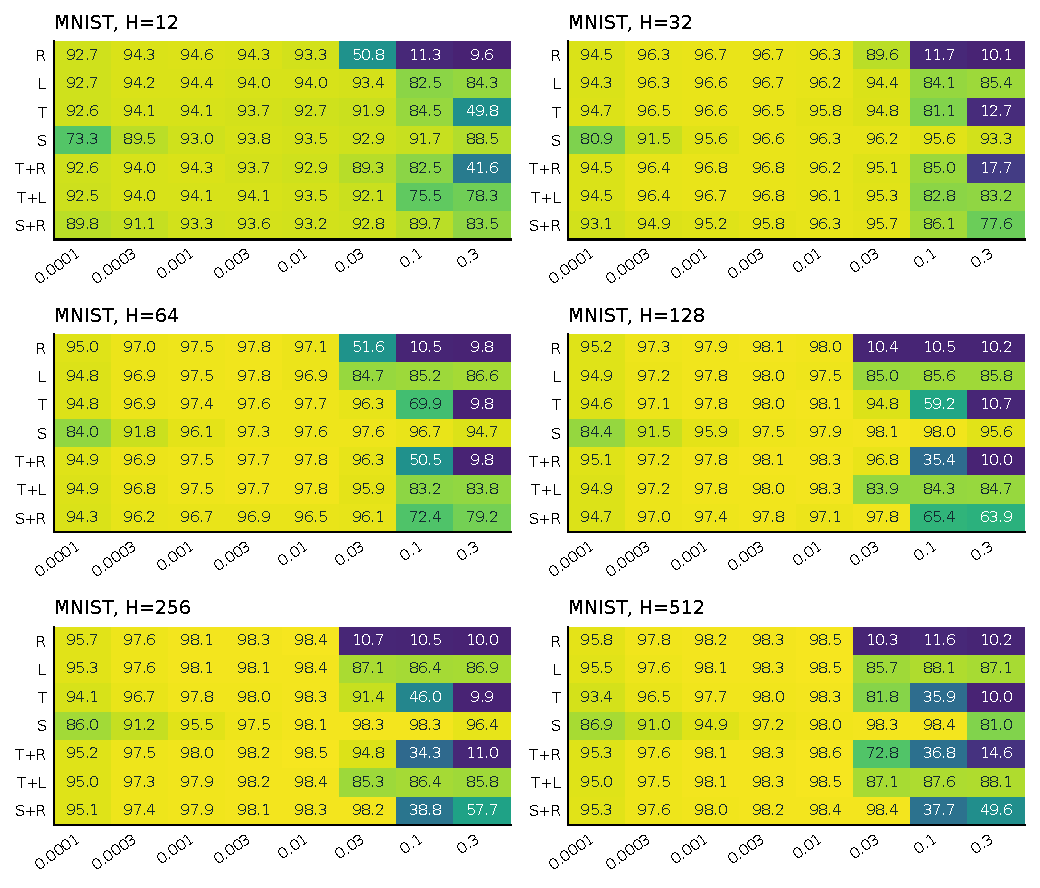
\includegraphics[width=\linewidth]{figures/calibration_ce_mnist.pdf}
\caption{MNIST CE calibration: mean final validation accuracy (\%) over six calibration seeds. Columns are learning rates; rows use the model codes given in Appendix~\ref{app:main}.}
\label{fig:calibrationce}\end{figure}
\begin{figure}[htbp]\centering
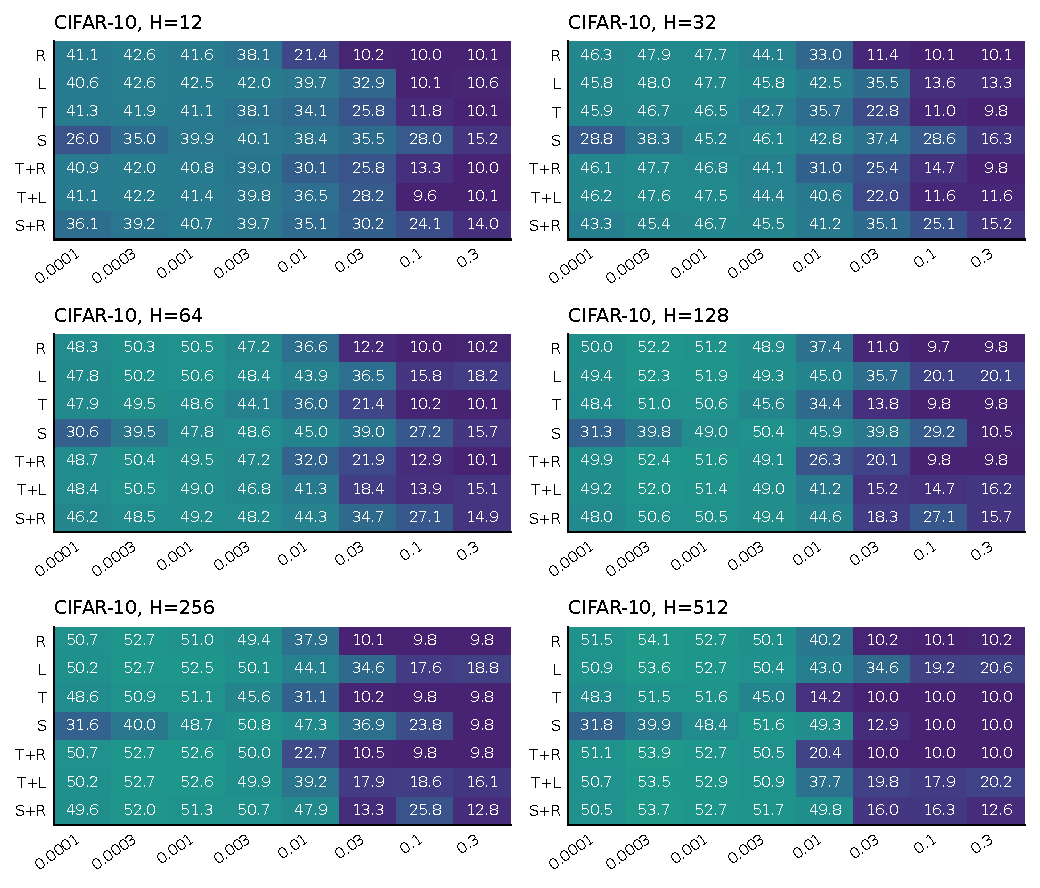
\includegraphics[width=\linewidth]{figures/calibration_ce_cifar10.pdf}
\caption{CIFAR-10 CE calibration: mean final validation accuracy (\%) over six calibration seeds. The color scale matches the MNIST calibration panels.}
\label{fig:calibrationcifar}\end{figure}
\begin{figure}[htbp]\centering
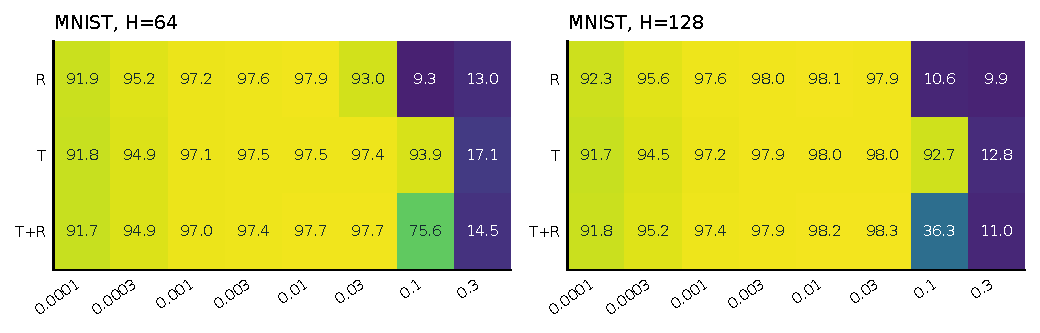
\includegraphics[width=\linewidth]{figures/calibration_mse.pdf}
\caption{MSE calibration means on MNIST, using the implemented sigmoid-output loss. Each cell contains six calibration seeds.}
\label{fig:calibrationmse}\end{figure}
\FloatBarrier

\section{Ratio and layout comparisons}\label{app:ratio}
The six ratio tests below have their own Holm correction. It covers neither the layout tests nor additional comparisons against pure-function controls. Random layouts change the subsequent random-number stream, as discussed in the main text. All ratio and layout tests use MNIST, H=128, and LR=0.01. The 50:50 interleave jobs repeat the corresponding main conditions and are not extra independent samples.
\begin{table}[htbp]
\centering
\caption{Paired ratio comparisons. Holm correction covers these six tests only.}
\label{tab:ratiopairs}
\footnotesize
\begin{tabular}{@{}llrrr@{}}
\toprule
Model & Ratio change & Difference (pp) & 95\% paired interval & Holm p \\
\midrule
tanh + leaky-ReLU & 0.25 to 0.50 & +0.021 & [-0.029, +0.068] & 0.811 \\
tanh + leaky-ReLU & 0.25 to 0.75 & +0.087 & [+0.051, +0.123] & 0.000478 \\
tanh + leaky-ReLU & 0.50 to 0.75 & +0.066 & [+0.025, +0.108] & 0.0153 \\
tanh + ReLU & 0.25 to 0.50 & +0.081 & [+0.036, +0.126] & 0.00702 \\
tanh + ReLU & 0.25 to 0.75 & +0.095 & [+0.050, +0.138] & 0.00182 \\
tanh + ReLU & 0.50 to 0.75 & +0.014 & [-0.016, +0.047] & 0.811 \\
\bottomrule
\end{tabular}
\end{table}

\begin{table}[htbp]
\centering
\caption{Mask layout at MNIST H=128, LR=0.01 and $\rho=0.5$. Differences use the interleave mask as the reference.}
\label{tab:layouts}
\footnotesize
\begin{tabular}{@{}llrrr@{}}
\toprule
Model & Layout & Accuracy (\%), mean $\pm$ SD & Difference (pp) & 95\% interval \\
\midrule
tanh + ReLU & interleave & 98.038 $\pm$ 0.073 & +0.000 & [+0.000, +0.000] \\
tanh + ReLU & block & 98.020 $\pm$ 0.088 & -0.018 & [-0.056, +0.021] \\
tanh + ReLU & random & 98.034 $\pm$ 0.108 & -0.004 & [-0.055, +0.046] \\
tanh + leaky-ReLU & interleave & 97.986 $\pm$ 0.081 & +0.000 & [+0.000, +0.000] \\
tanh + leaky-ReLU & block & 98.022 $\pm$ 0.086 & +0.036 & [-0.013, +0.085] \\
tanh + leaky-ReLU & random & 98.017 $\pm$ 0.071 & +0.031 & [-0.000, +0.066] \\
\bottomrule
\end{tabular}
\end{table}

\FloatBarrier

\section{Training gaps and class-level recall}\label{app:classes}
Figure~\ref{fig:gaps} matches the clean training score to each run's selected epoch. It does not subtract the final-epoch training score from a different checkpoint's test score. The training subset has 10,000 fixed images. These gaps show a larger train--test difference as CIFAR-10 width grows.
\begin{figure}[htbp]\centering
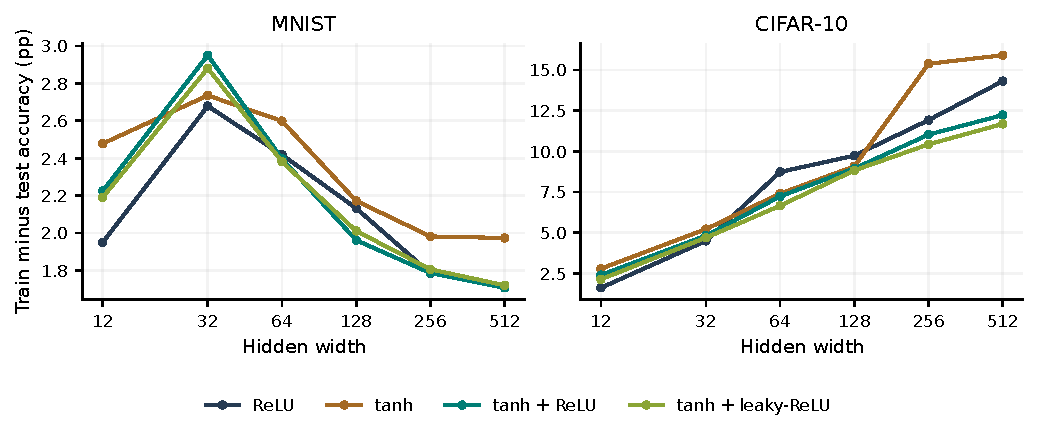
\includegraphics[width=\linewidth]{figures/train_test_gap.pdf}
\caption{Mean clean training accuracy minus test accuracy at the selected checkpoint. The gap grows with width on CIFAR-10. It remains much smaller on MNIST.}
\label{fig:gaps}\end{figure}

Class recall in Figure~\ref{fig:classes} is the share of each true class that is correctly predicted, averaged across seeds. It shows details hidden by an overall score, but the figure is descriptive. Shared test images mean that predictions from different seeds are not independent test datasets. Confusion matrices also do not retain the per-image disagreements needed for a paired test across images.
\begin{figure}[htbp]\centering
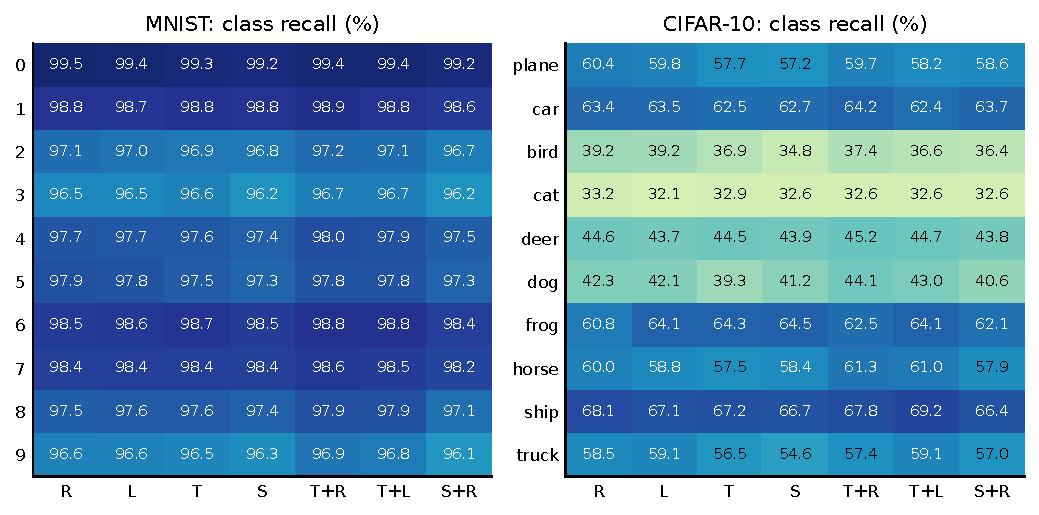
\includegraphics[width=\linewidth]{figures/class_recall.pdf}
\caption{Per-class recall at H=128 for all seven main models. Every cell is a mean across 30 selected checkpoints. The two panels use different color ranges (MNIST: 90--100\%; CIFAR-10: 20--80\%); numbers show the measured values. Model codes follow Appendix~\ref{app:main}.}
\label{fig:classes}\end{figure}
\FloatBarrier
\end{document}
